%% LyX 1.3 created this file.  For more info, see http://www.lyx.org/.
%% Do not edit unless you really know what you are doing.
\documentclass[12pt,english]{article}
\usepackage[T1]{fontenc}
\usepackage[latin1]{inputenc}
\usepackage{graphicx}

\makeatletter

%%%%%%%%%%%%%%%%%%%%%%%%%%%%%% LyX specific LaTeX commands.
\newcommand{\noun}[1]{\textsc{#1}}
%% Bold symbol macro for standard LaTeX users
\providecommand{\boldsymbol}[1]{\mbox{\boldmath $#1$}}


%%%%%%%%%%%%%%%%%%%%%%%%%%%%%% Textclass specific LaTeX commands.
 \newenvironment{lyxlist}[1]
   {\begin{list}{}
     {\settowidth{\labelwidth}{#1}
      \setlength{\leftmargin}{\labelwidth}
      \addtolength{\leftmargin}{\labelsep}
      \renewcommand{\makelabel}[1]{##1\hfil}}}
   {\end{list}}

%%%%%%%%%%%%%%%%%%%%%%%%%%%%%% User specified LaTeX commands.
\usepackage[T1]{fontenc}
\usepackage[latin1]{inputenc}
\usepackage{geometry}
\geometry{verbose,a4paper,lmargin=2.5cm,rmargin=2cm}
\usepackage{babel}
\usepackage{graphics}
\usepackage{setspace}

\usepackage{babel}
\makeatother
\begin{document}

\title{ParaGauss Molecular Mechanics module\\
{\normalsize version 0.95}\\
(user manual) }


\author{Aleksey Shor}

\maketitle

\section{Force field}

~~~~~The force field is the set of analytical and tabulated potential
functions which need to define interactions into a molecular system.
The potential functions implemented in Molecular mechanics module
can be divided in two parts: 

\begin{enumerate}
\item \textit{Bonded (covalent interactions)} : stretching, bending, torsion
and cross terms (stretching-stretching, bending-bending, stretching-bending,
stretching-torsion) and also core-shell interaction
\item \textit{Non-bonded (van der Waals and electrostatic interactions)}
: Lennard-Jones, Buckingham, point charges, dipole-dipole and tabulated. 
\end{enumerate}

\subsection{Bonded interactions }


\subsubsection{Stretching potentials}

\begin{center}\textbf{\includegraphics{mm0a.eps}}\end{center}

Harmonic\begin{equation}
E\left(r_{ij}\right)=\frac{k2_{ij}}{2}\left(r_{ij}-r_{ij}^{0}\right)^{2}\label{eq:1}\end{equation}


Quartic\begin{eqnarray}
E\left(r_{ij}\right) & = & \frac{k2_{ij}}{2}\left(r_{ij}-r_{ij}^{0}\right)^{2}+\frac{k3_{ij}}{3}\left(r_{ij}-r_{ij}^{0}\right)^{3}\nonumber \\
 & + & \frac{k4_{ij}}{4}\left(r_{ij}-r_{ij}^{0}\right)^{4}\label{eq:2}\end{eqnarray}


Morse\begin{equation}
E\left(r_{ij}\right)=D_{ij}\left\{ \left[1-\exp\left(-A_{ij}\left(r_{ij}-r_{ij}^{0}\right)\right)\right]^{2}-1\right\} \label{eq:3}\end{equation}


Buchingham\begin{equation}
E\left(r_{ij}\right)=A_{ij}\exp\left(-\frac{r_{ij}}{\rho_{ij}}\right)-\frac{C_{ij}}{r_{ij}^{6}}\label{eq:22}\end{equation}



\subsubsection{Bending potentials}

\begin{center}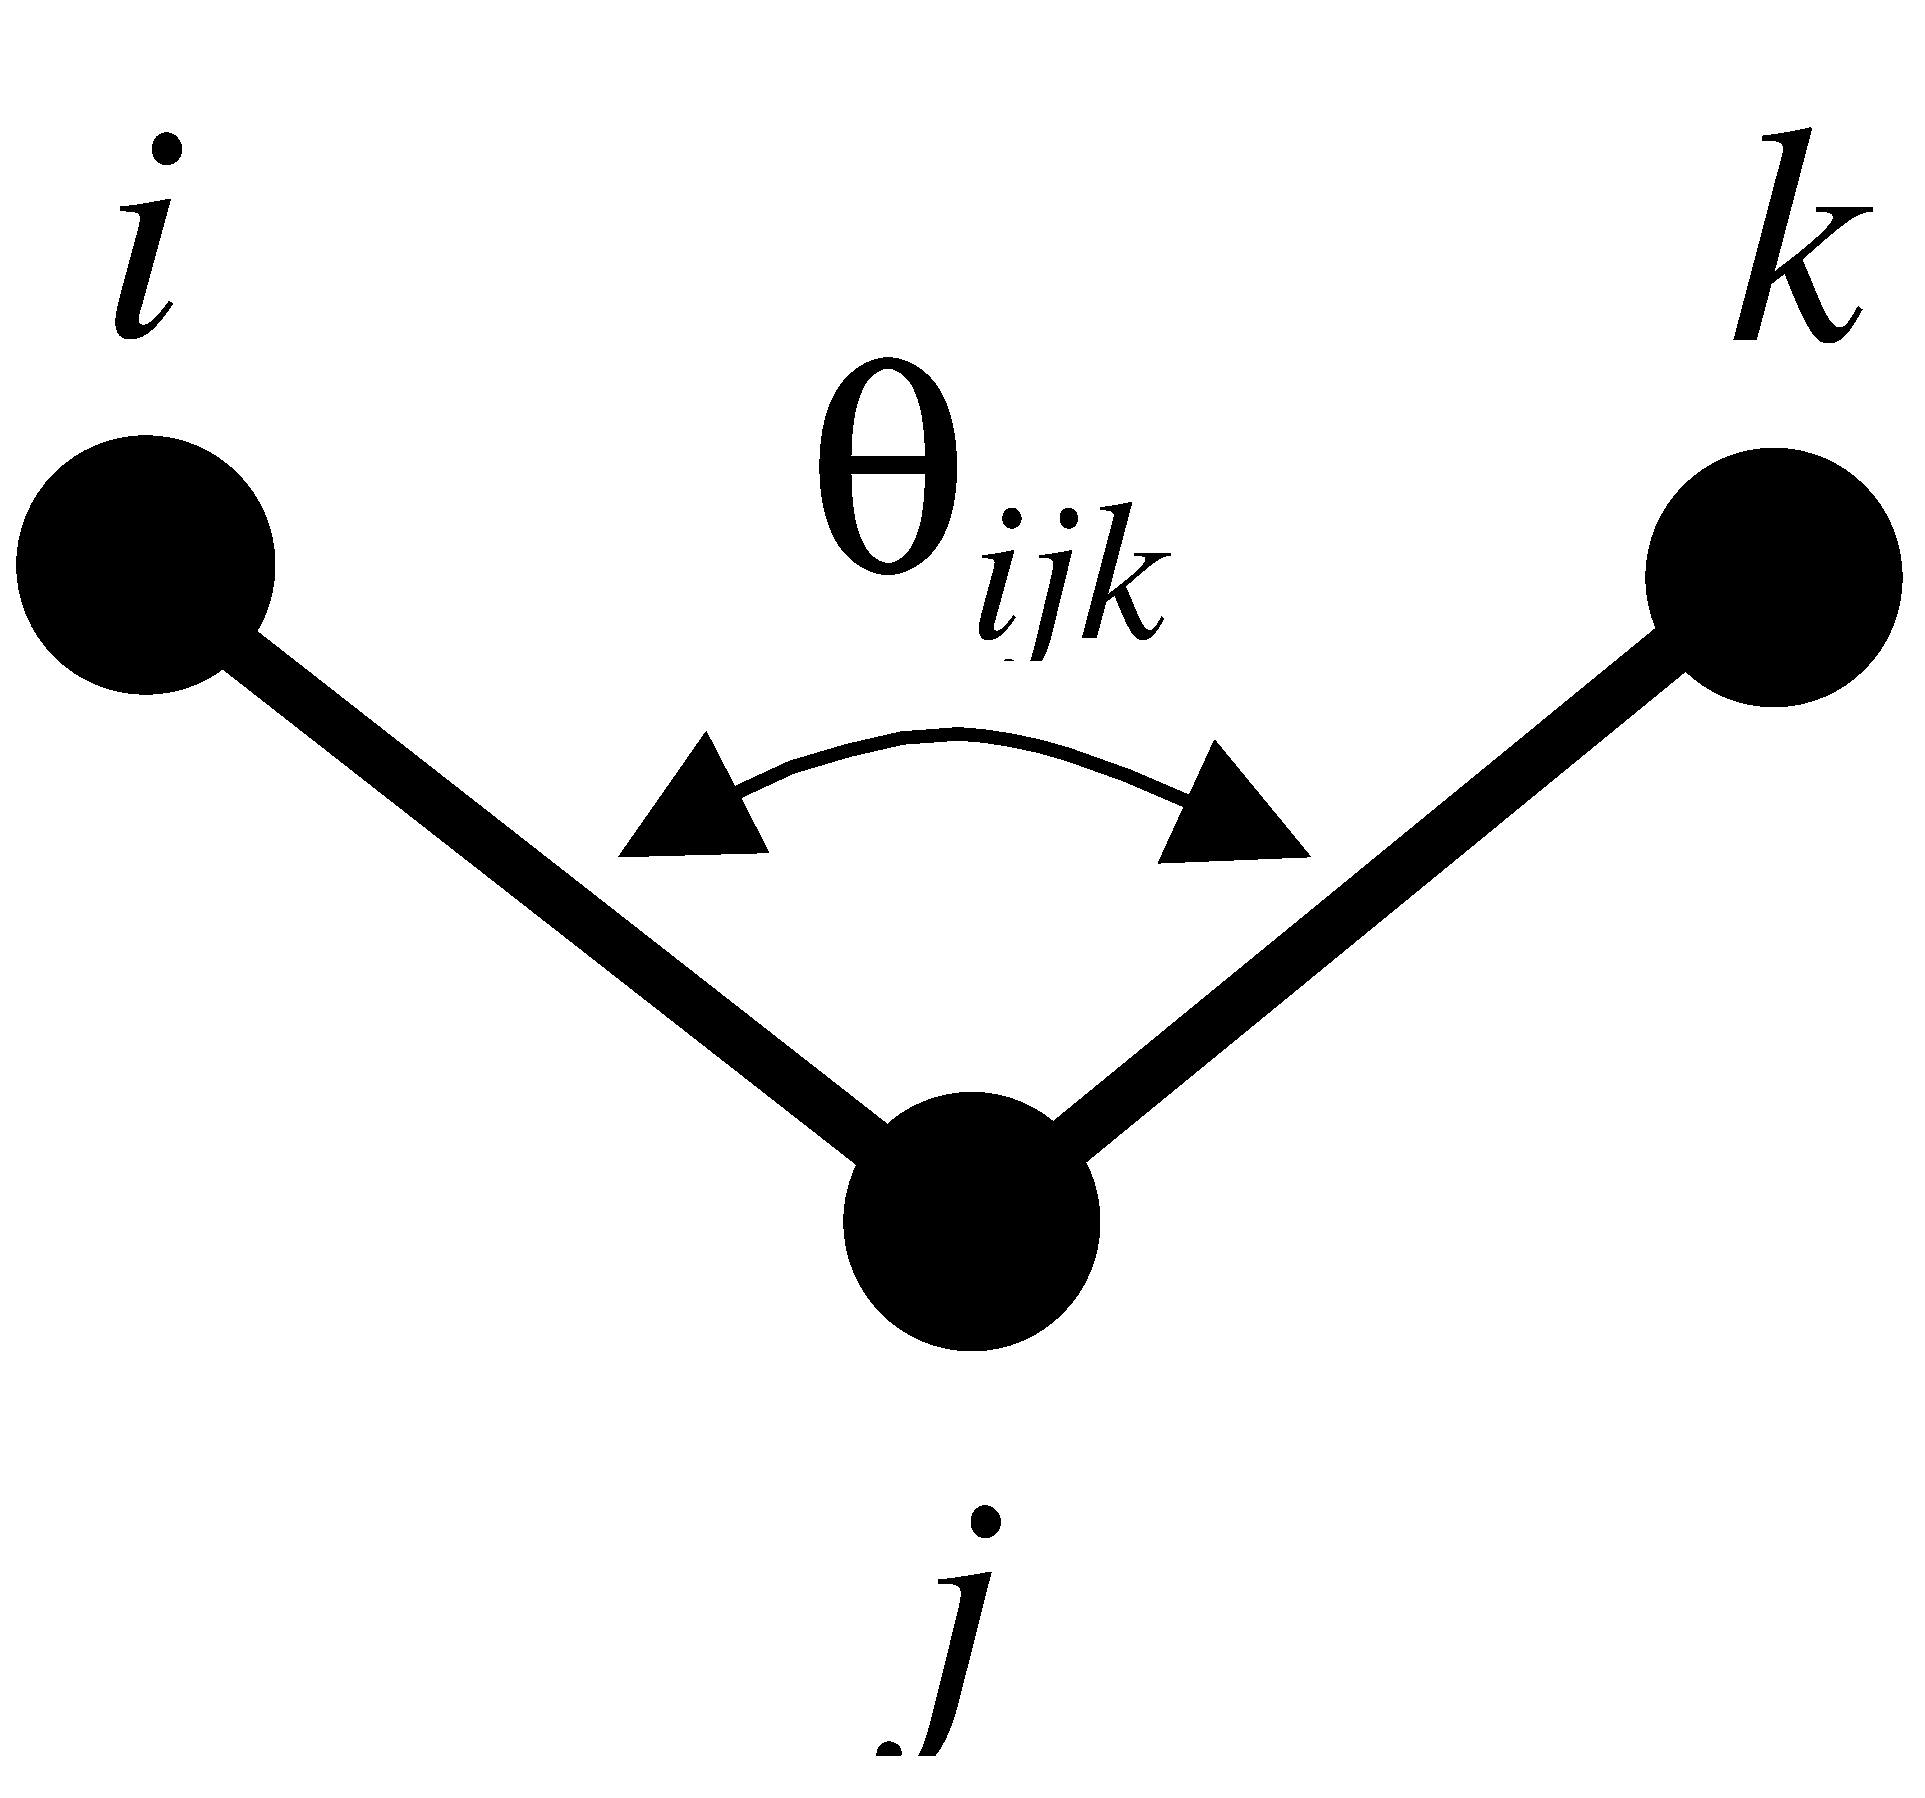
\includegraphics[%
  width=4cm,
  height=3.5cm]{mm1.eps}\end{center}

Harmonic\begin{equation}
E\left(\theta_{ijk}\right)=\frac{k2_{ijk}}{2}\left(\theta_{ijk}-\theta_{ijk}^{0}\right)^{2}\label{eq:4}\end{equation}


Quartic\begin{eqnarray}
E\left(\theta_{ijk}\right) & = & \frac{k2_{ijk}}{2}\left(\theta_{ijk}-\theta_{ijk}^{0}\right)^{2}+\frac{k3_{ijk}}{3}\left(\theta_{ijk}-\theta_{ijk}^{0}\right)^{4}\nonumber \\
 & + & \frac{k4_{ijk}}{4}\left(\theta_{ijk}-\theta_{ijk}^{0}\right)^{4}\label{eq:5}\end{eqnarray}


Six \begin{eqnarray}
E\left(\theta_{ijk}\right) & = & \frac{k2_{ijk}}{2}\left(\theta_{ijk}-\theta_{ijk}^{0}\right)^{2}+\frac{k3_{ijk}}{3}\left(\theta_{ijk}-\theta_{ijk}^{0}\right)^{4}\label{eq:6}\\
 & + & \frac{k4_{ijk}}{4}\left(\theta_{ijk}-\theta_{ijk}^{0}\right)^{4}+\frac{k5_{ijk}}{5}\left(\theta_{ijk}-\theta_{ijk}^{0}\right)^{5}\nonumber \\
 & + & \frac{k6_{ijk}}{6}\left(\theta_{ijk}-\theta_{ijk}^{0}\right)^{6}\nonumber \\
\nonumber \end{eqnarray}



\subsubsection{Torsion potentials}

\begin{center}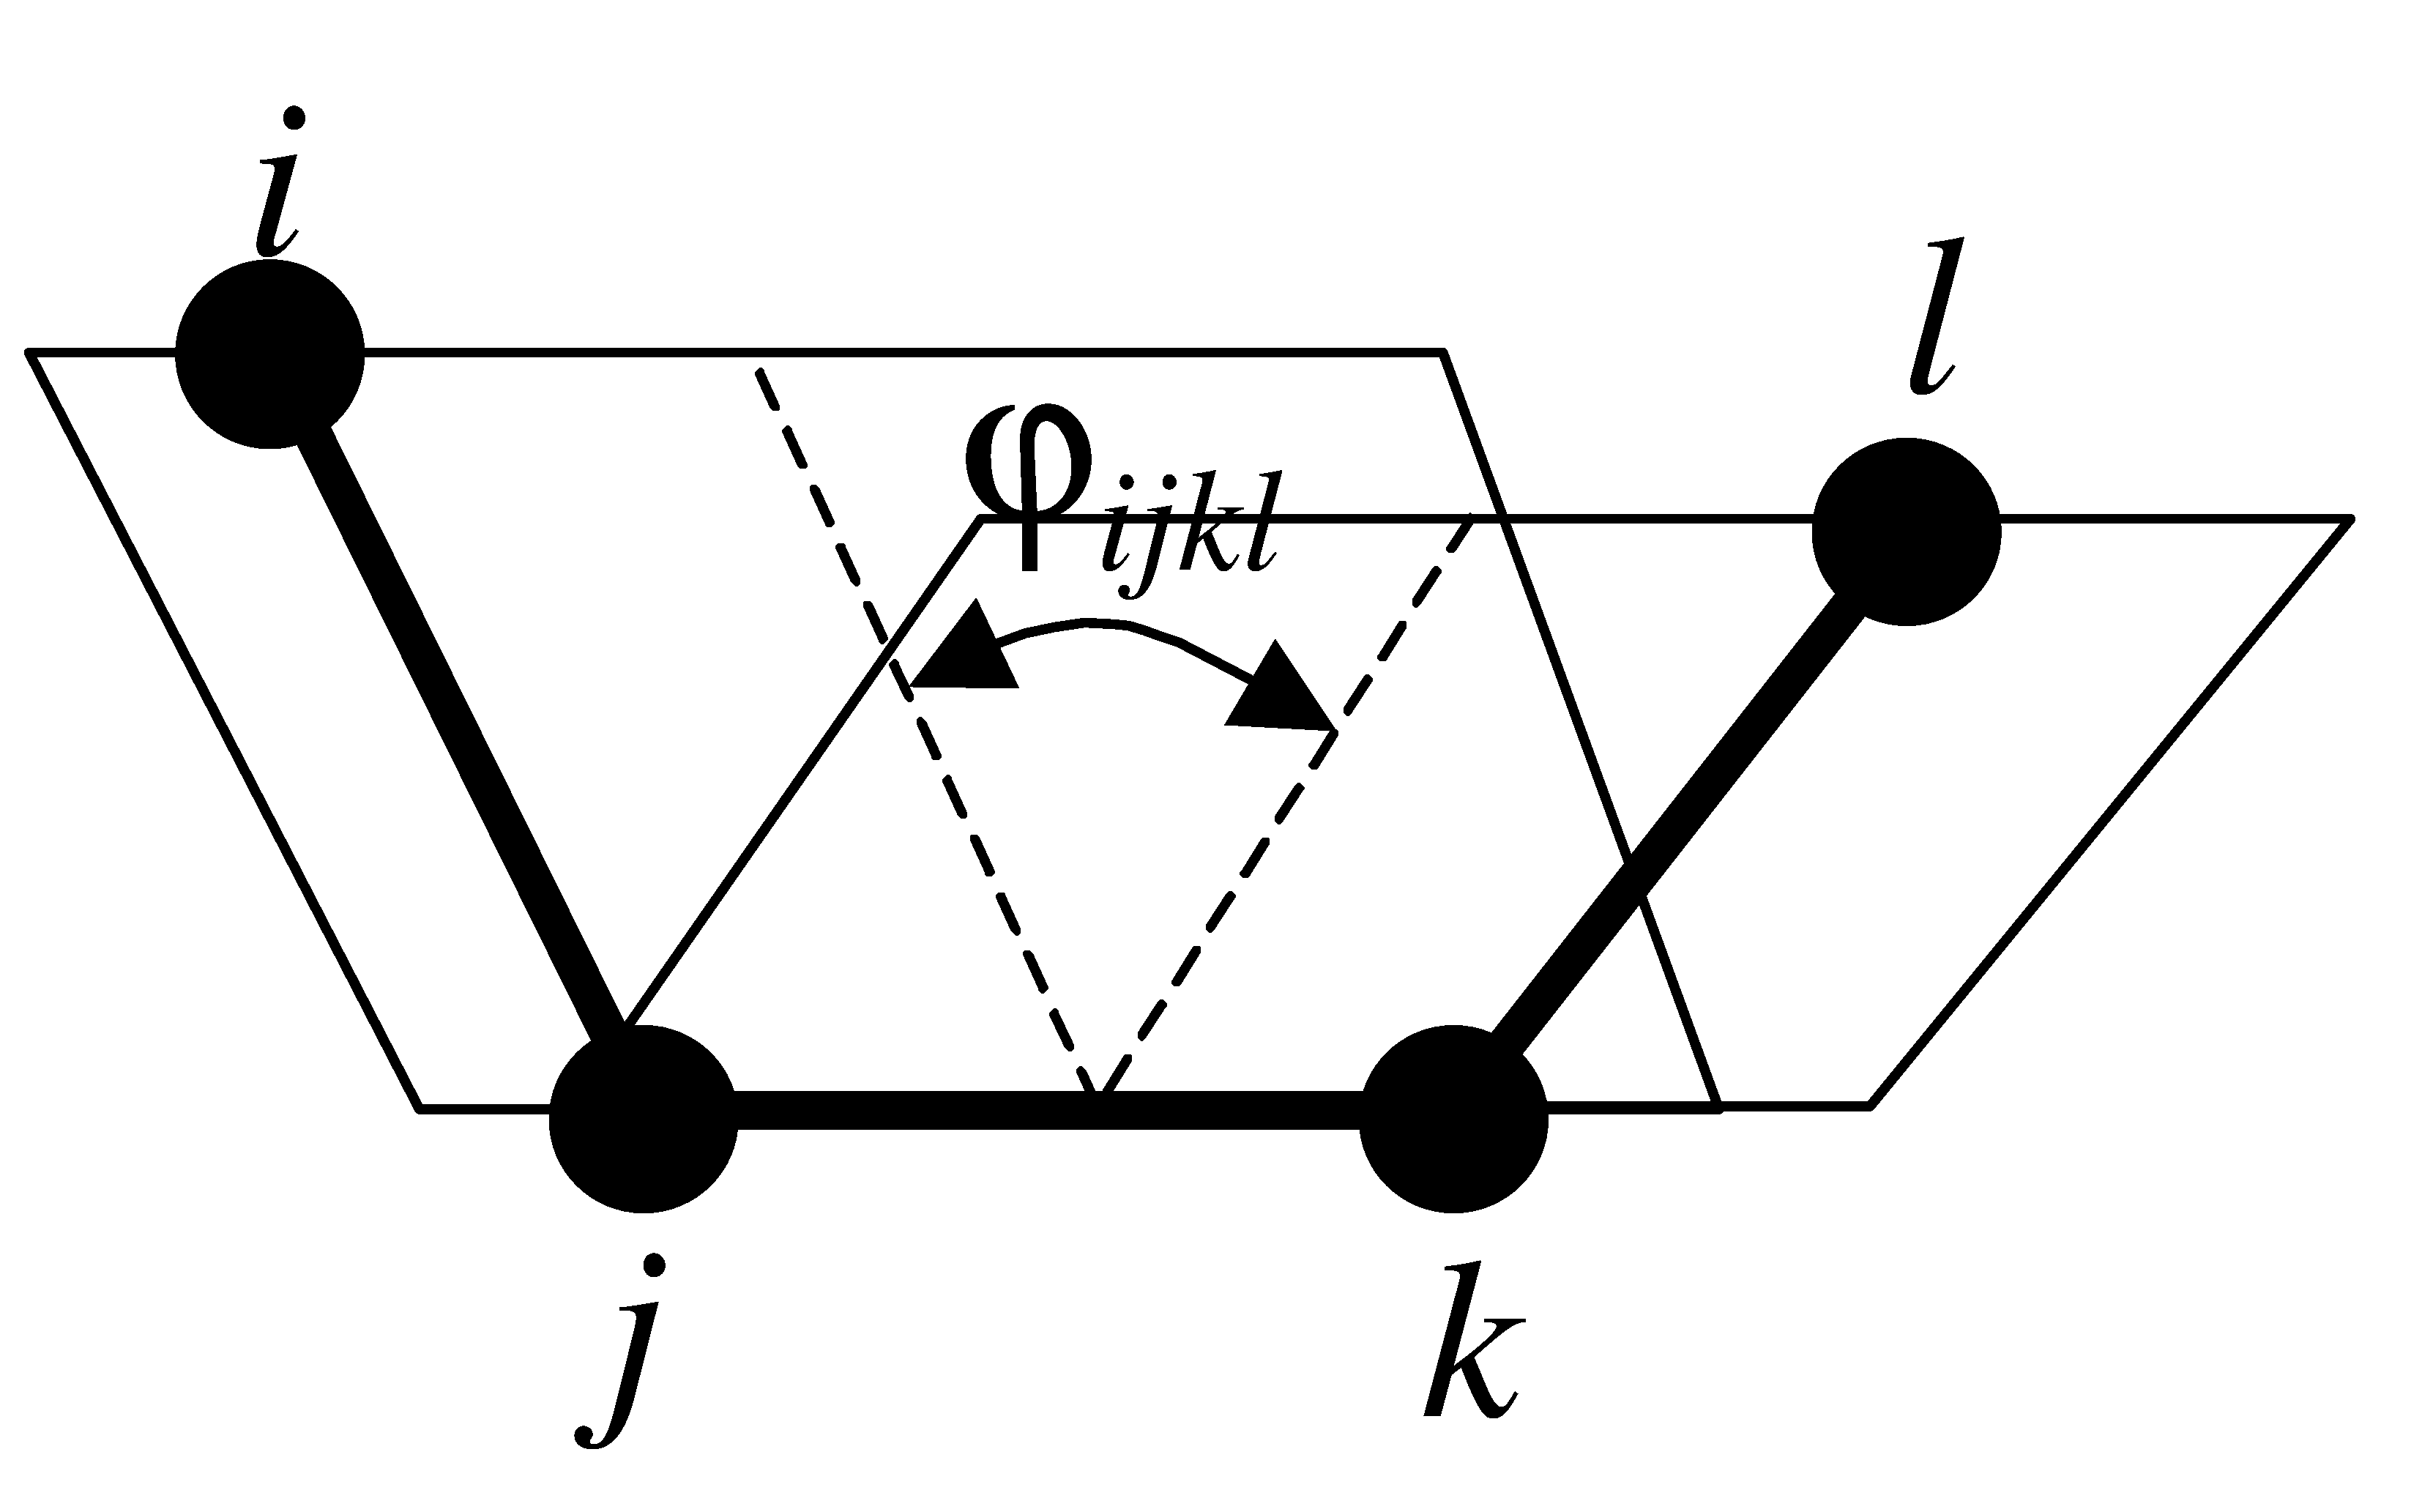
\includegraphics[%
  width=6cm,
  height=3.5cm]{mm2.eps}\end{center}

Harmonic\begin{equation}
E\left(\varphi_{ijkl}\right)=\frac{k2_{ijkl}}{2}\left(\varphi_{ijkl}-\varphi_{ijkl}^{0}\right)^{2}\label{eq:7}\end{equation}


Triple cosine\begin{eqnarray}
E\left(\varphi_{ijkl}\right) & = & \frac{k1_{ijkl}}{2}\left[1+\cos\left(\varphi_{ijkl}\right)\right]\nonumber \\
 & + & \frac{k2_{ijkl}}{2}\left[1-\cos\left(2\varphi_{ijkl}\right)\right]\label{eq:8}\\
 & + & \frac{k3_{ijkl}}{2}\left[1+\cos\left(3\varphi_{ijkl}\right)\right]\nonumber \\
\nonumber \end{eqnarray}



\subsubsection{Cross terms}

~~~~Stretching-stretching

\begin{center}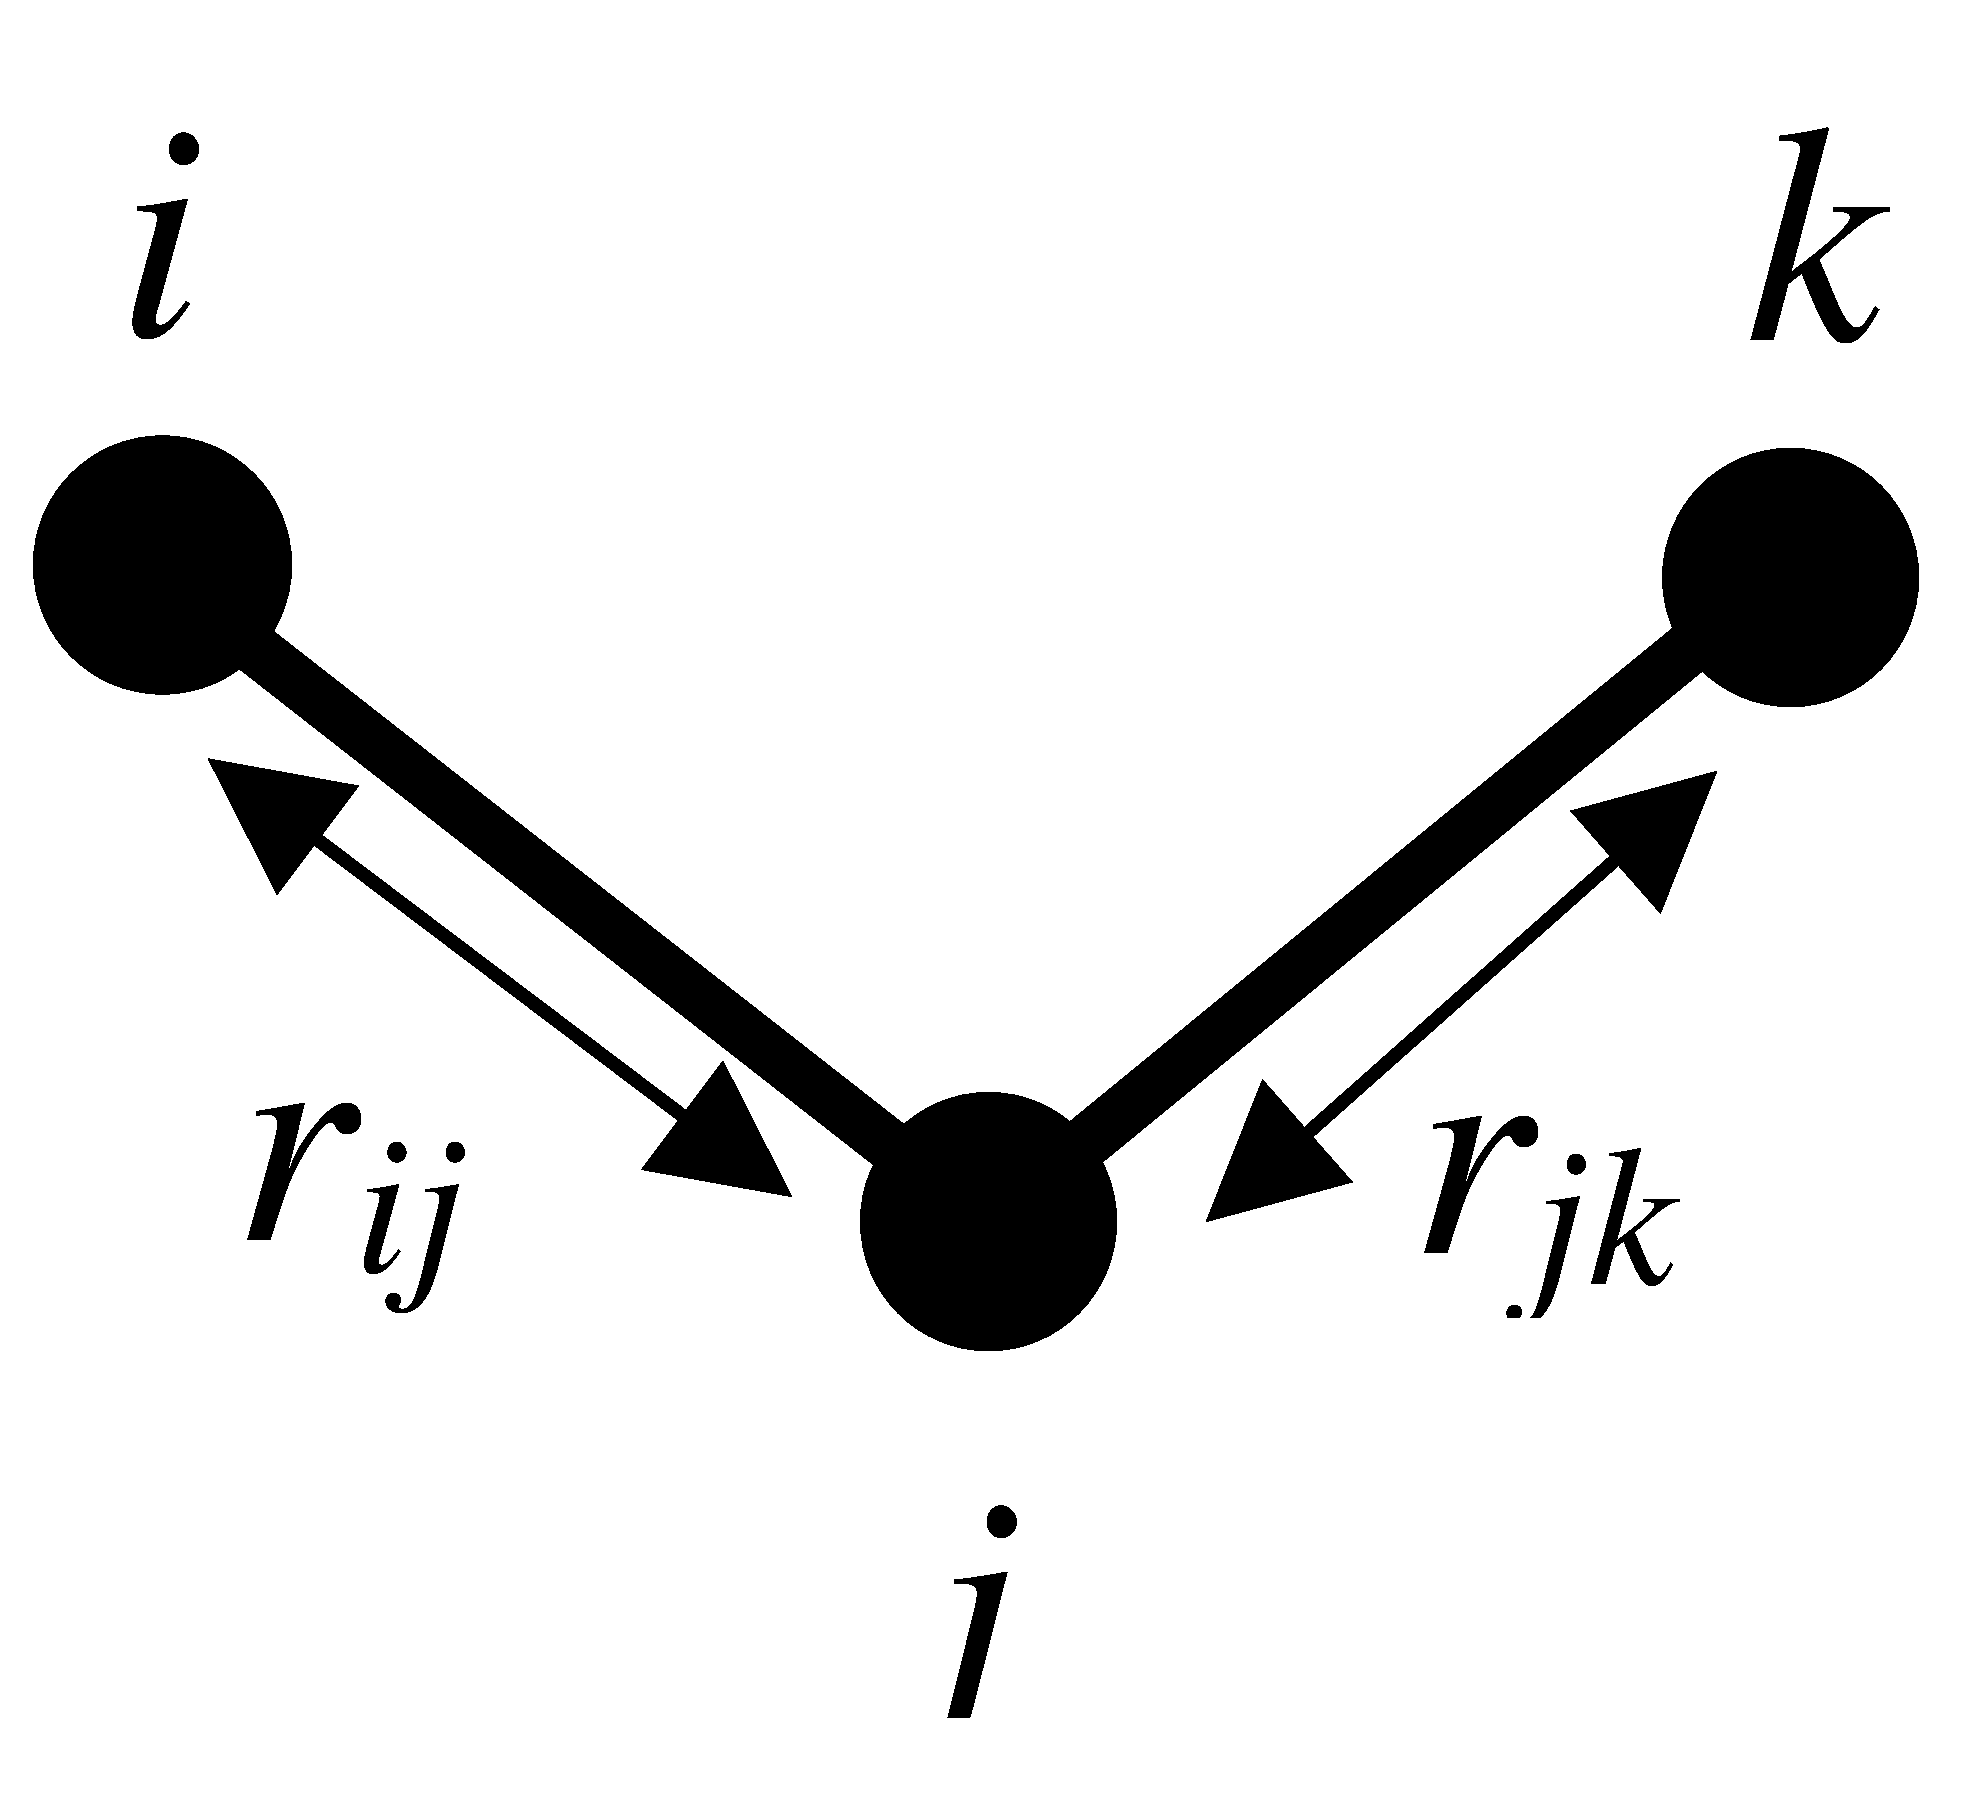
\includegraphics[%
  width=4cm,
  height=3.5cm]{mm3.eps}\begin{equation}
E\left(r_{ij},r_{kj}\right)=\frac{k_{ijk}}{2}\left(r_{ij}-r_{ij}^{0}\right)\left(r_{kj}-r_{kj}^{0}\right)\label{eq:9}\end{equation}
\end{center}

Bending-bending

\begin{center}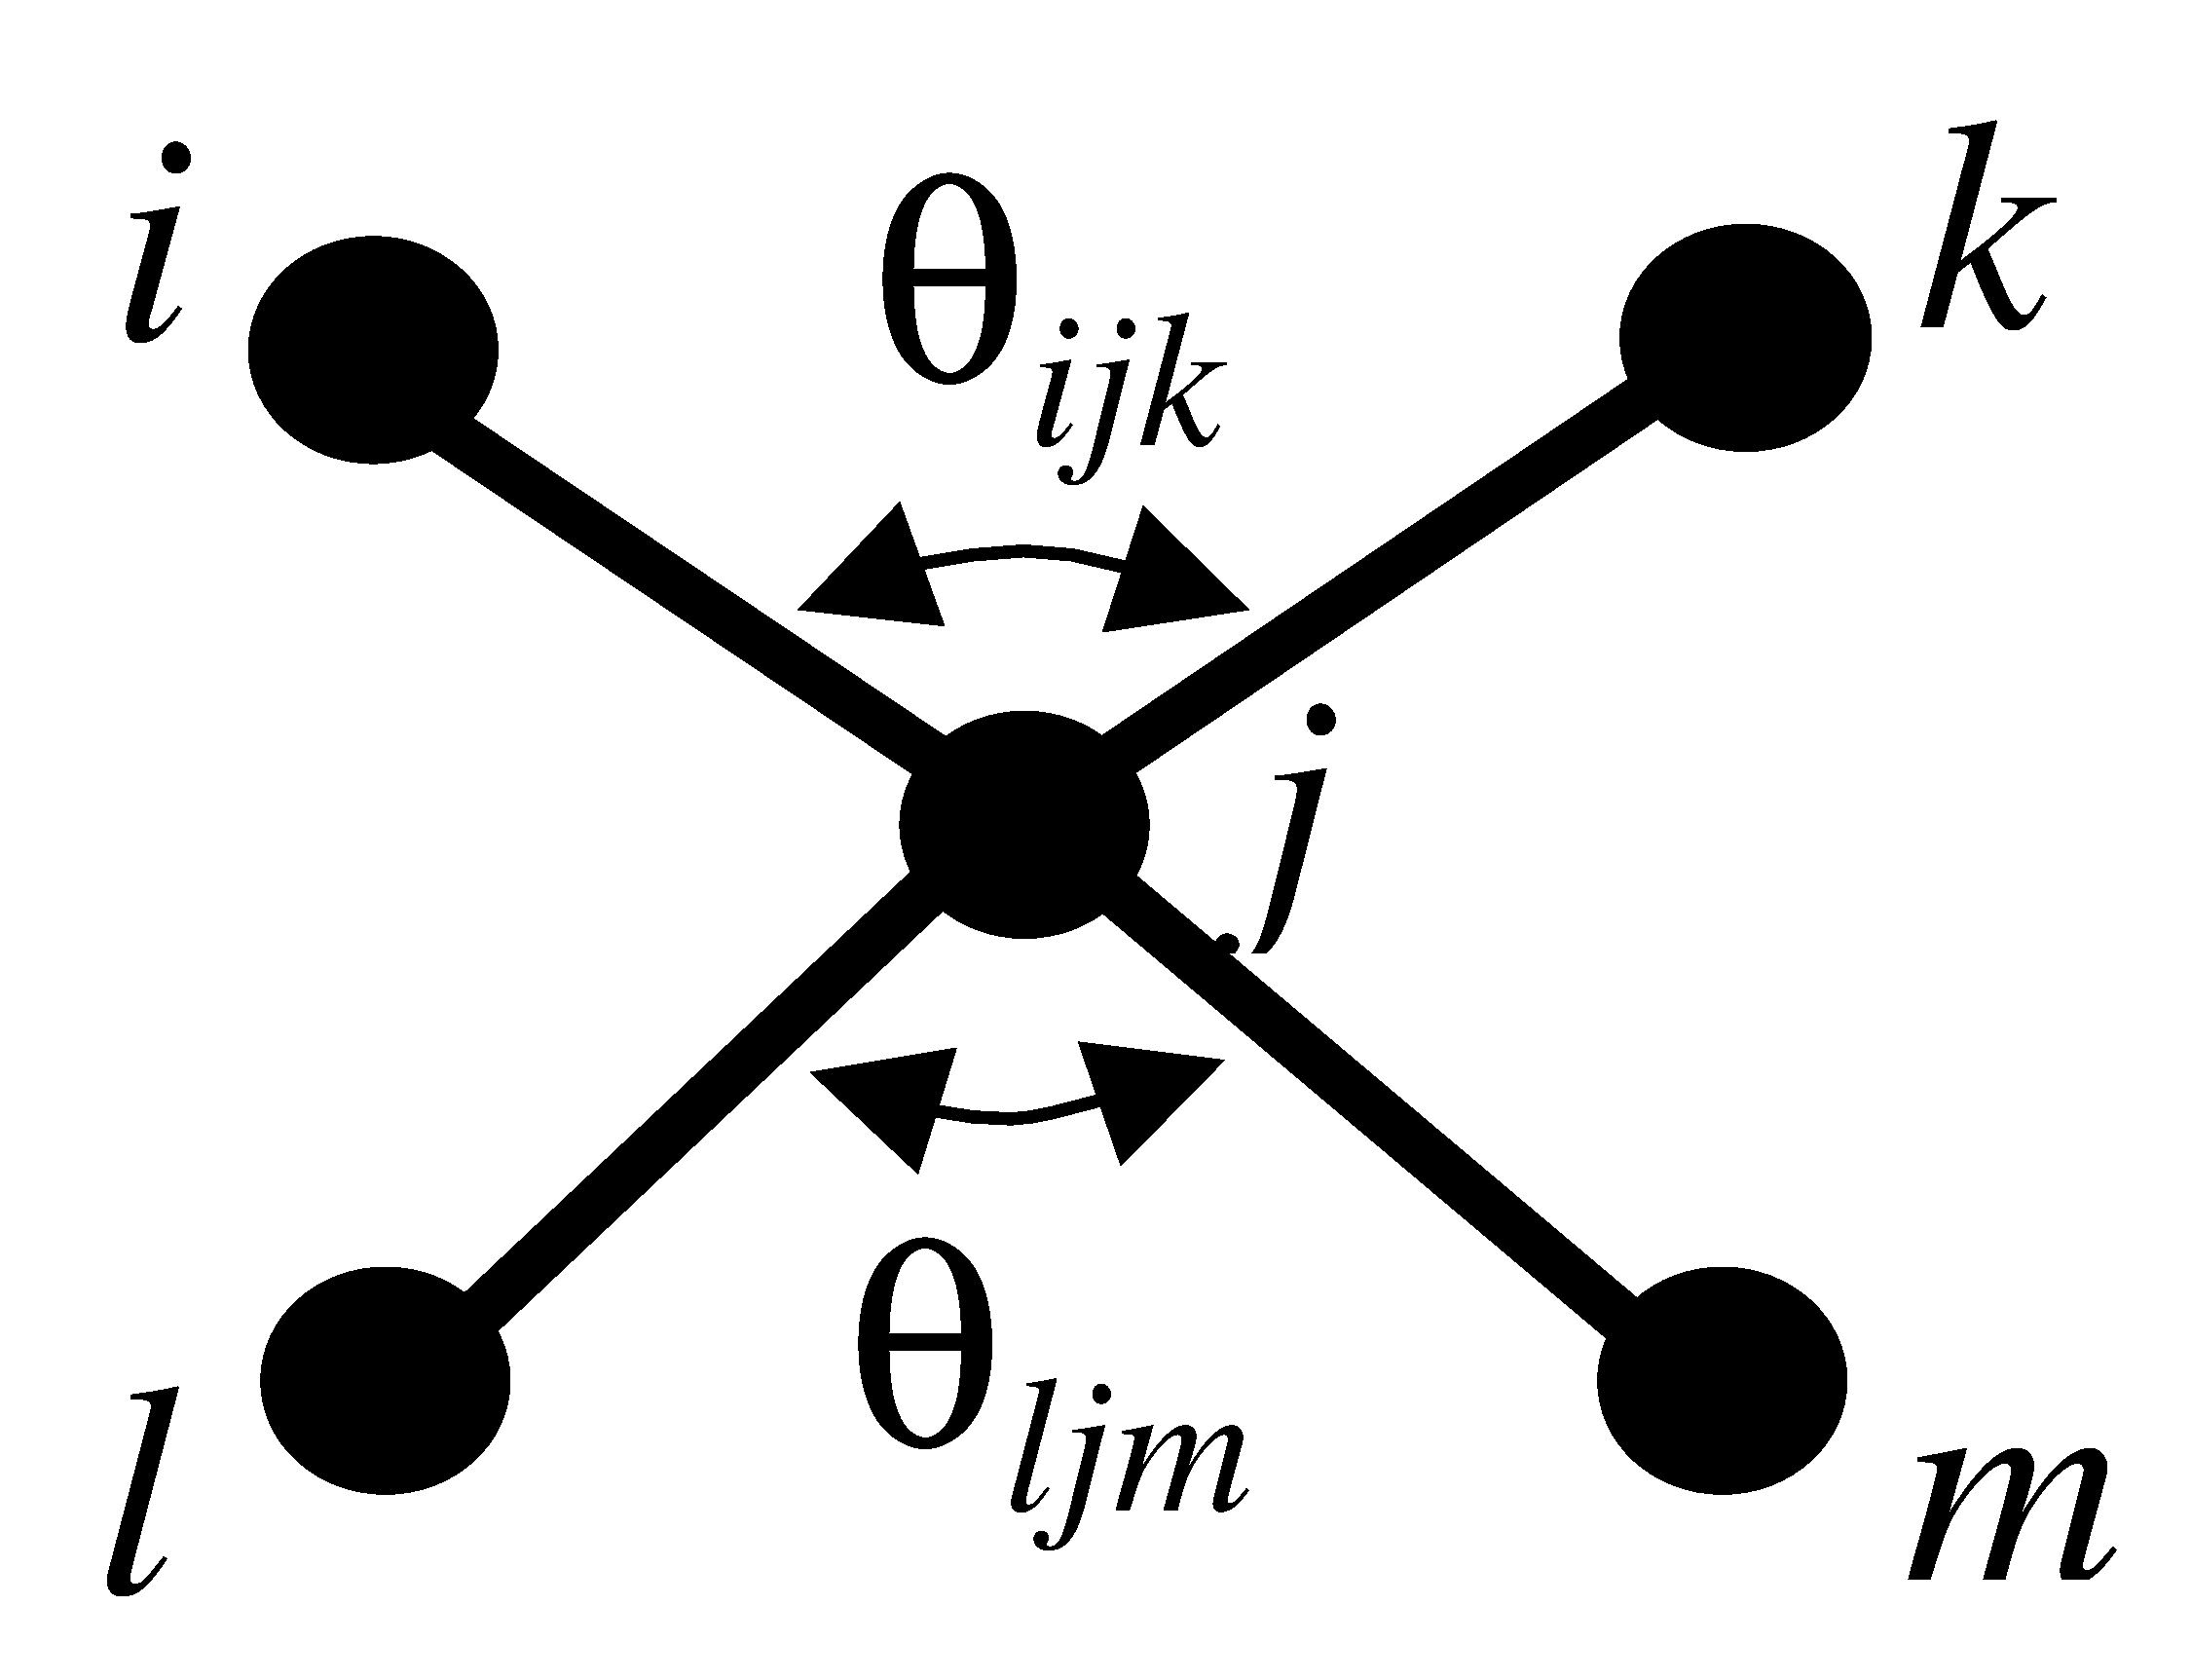
\includegraphics[%
  width=4cm,
  height=3.5cm]{mm4.eps}~~ or ~~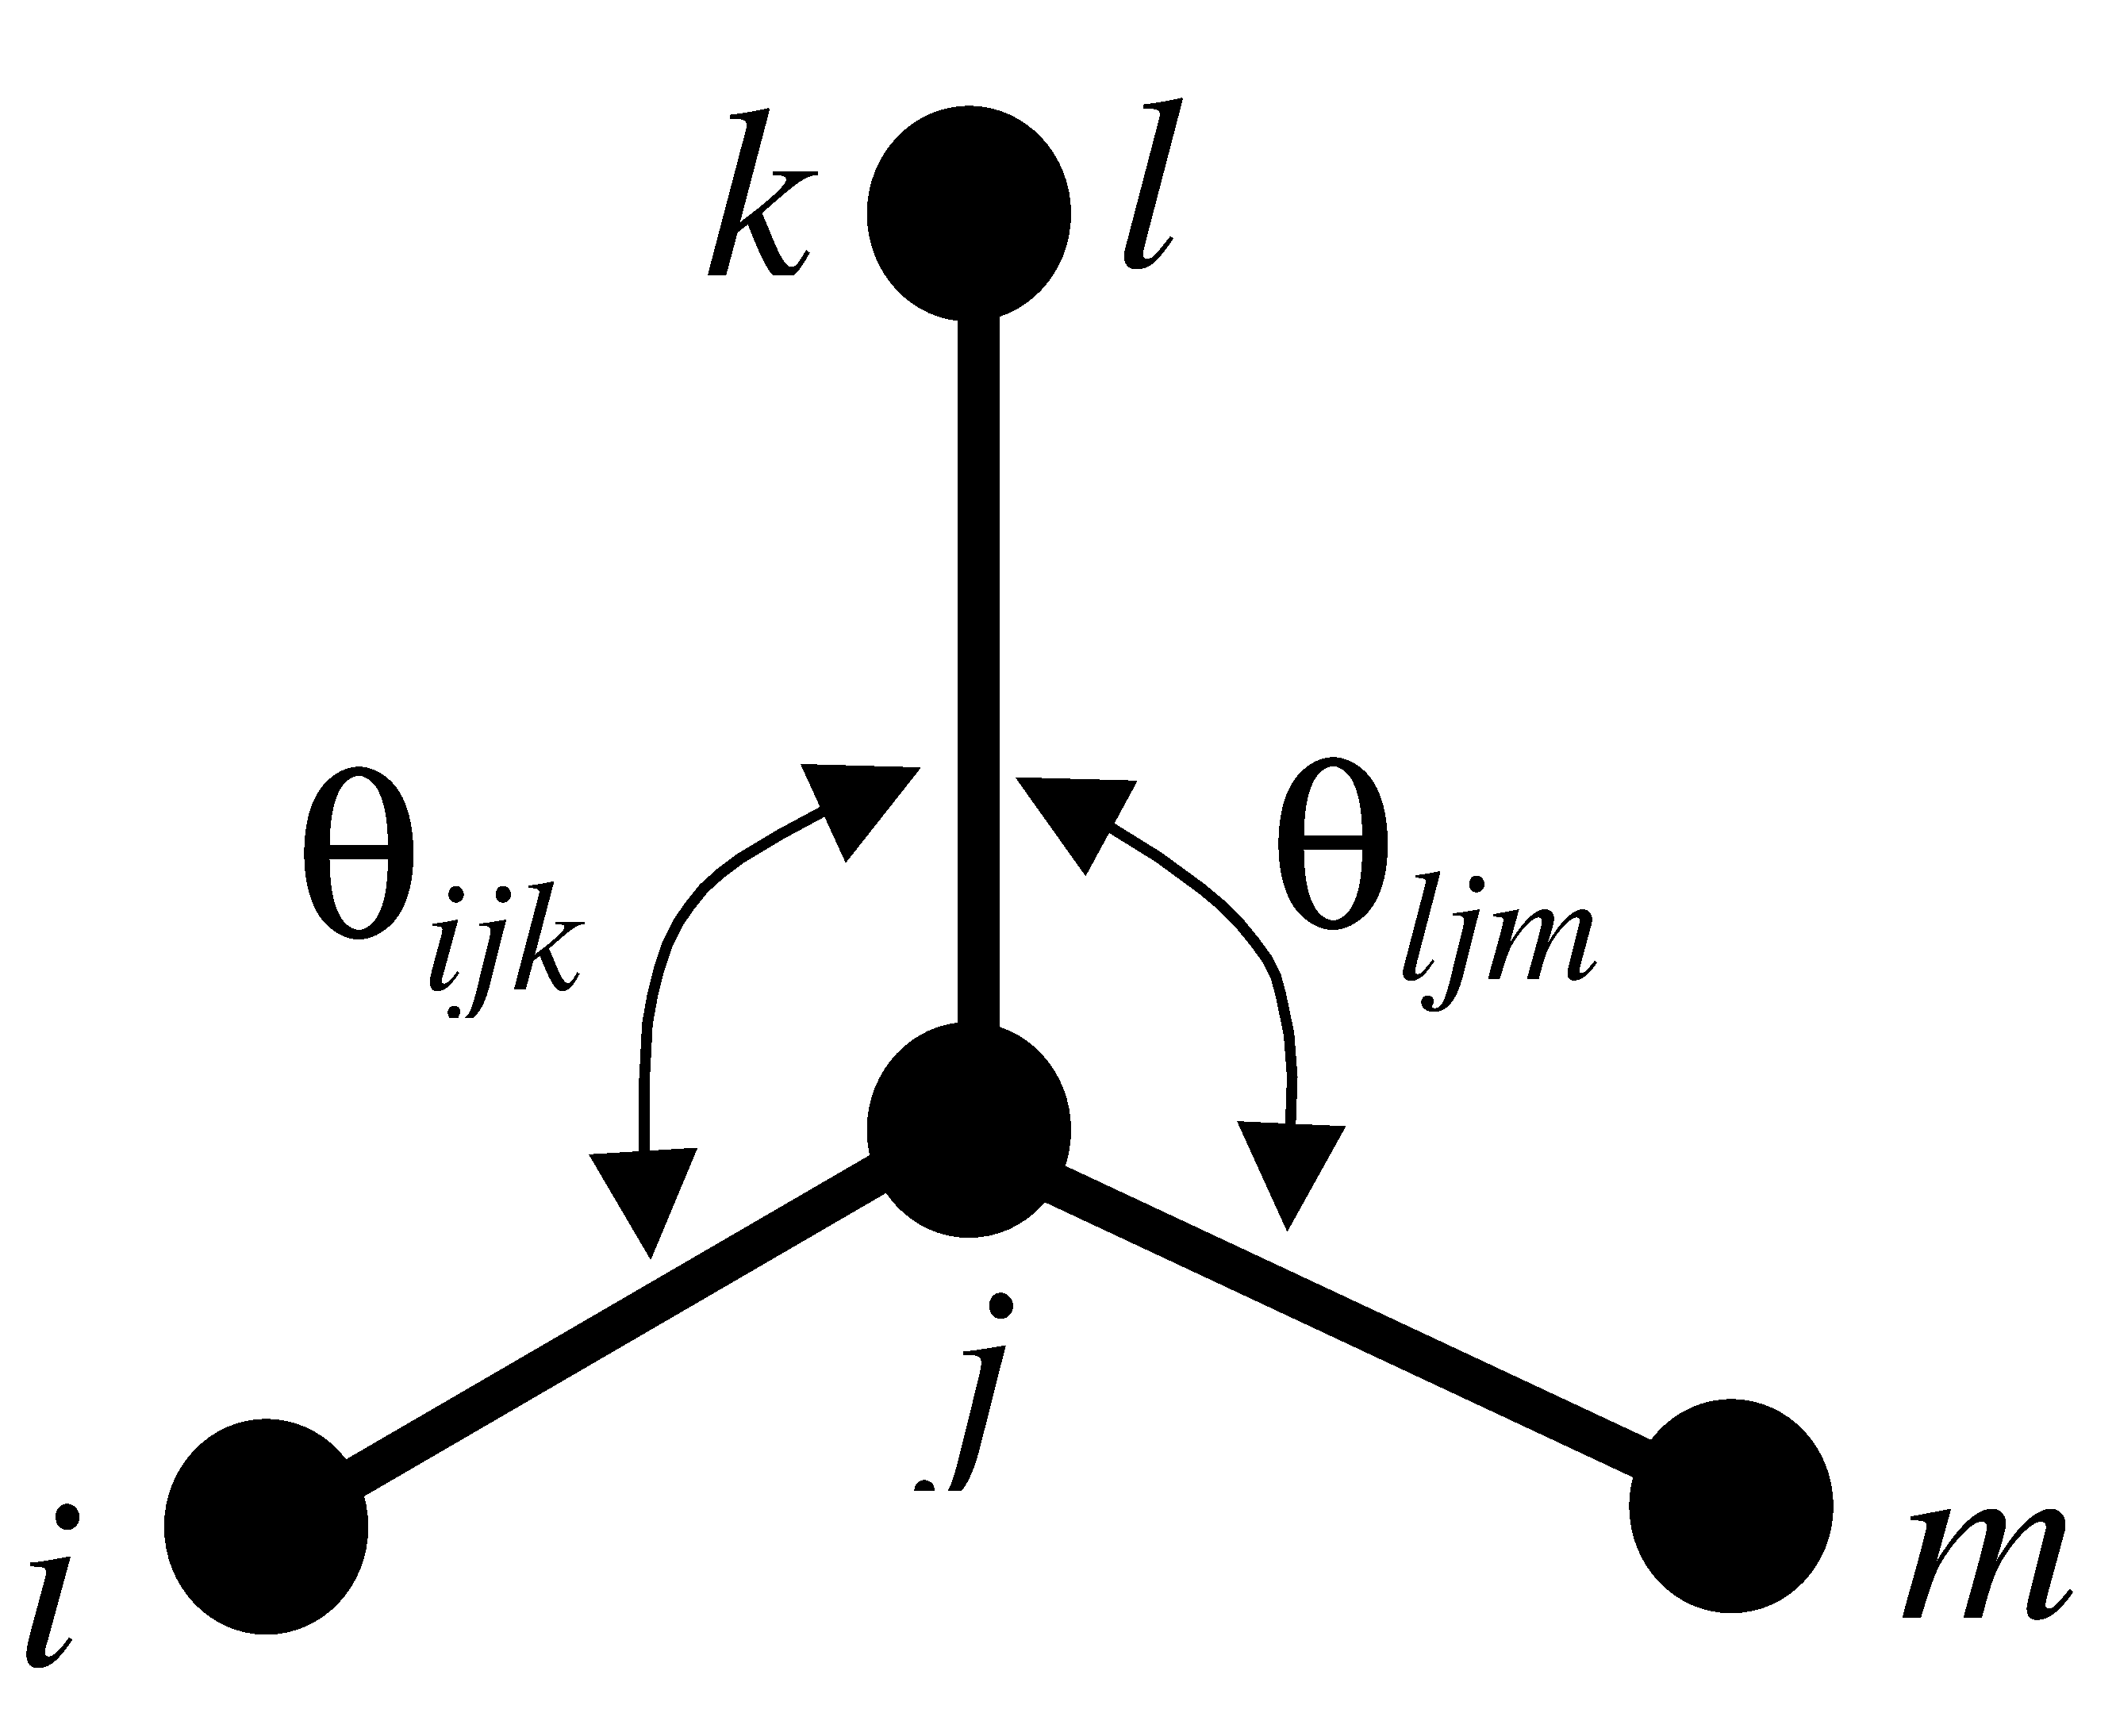
\includegraphics[%
  width=4cm,
  height=3.5cm]{mm5.eps}\begin{equation}
E\left(\theta_{ijk},\theta_{ljm}\right)=\frac{k_{ikjlm}}{2}\left(\theta_{ijk}-\theta_{ijk}^{0}\right)\left(\theta_{ljm}-\theta_{ljm}^{0}\right)\label{eq:10}\end{equation}
\end{center}

Stretching-bending

\begin{center}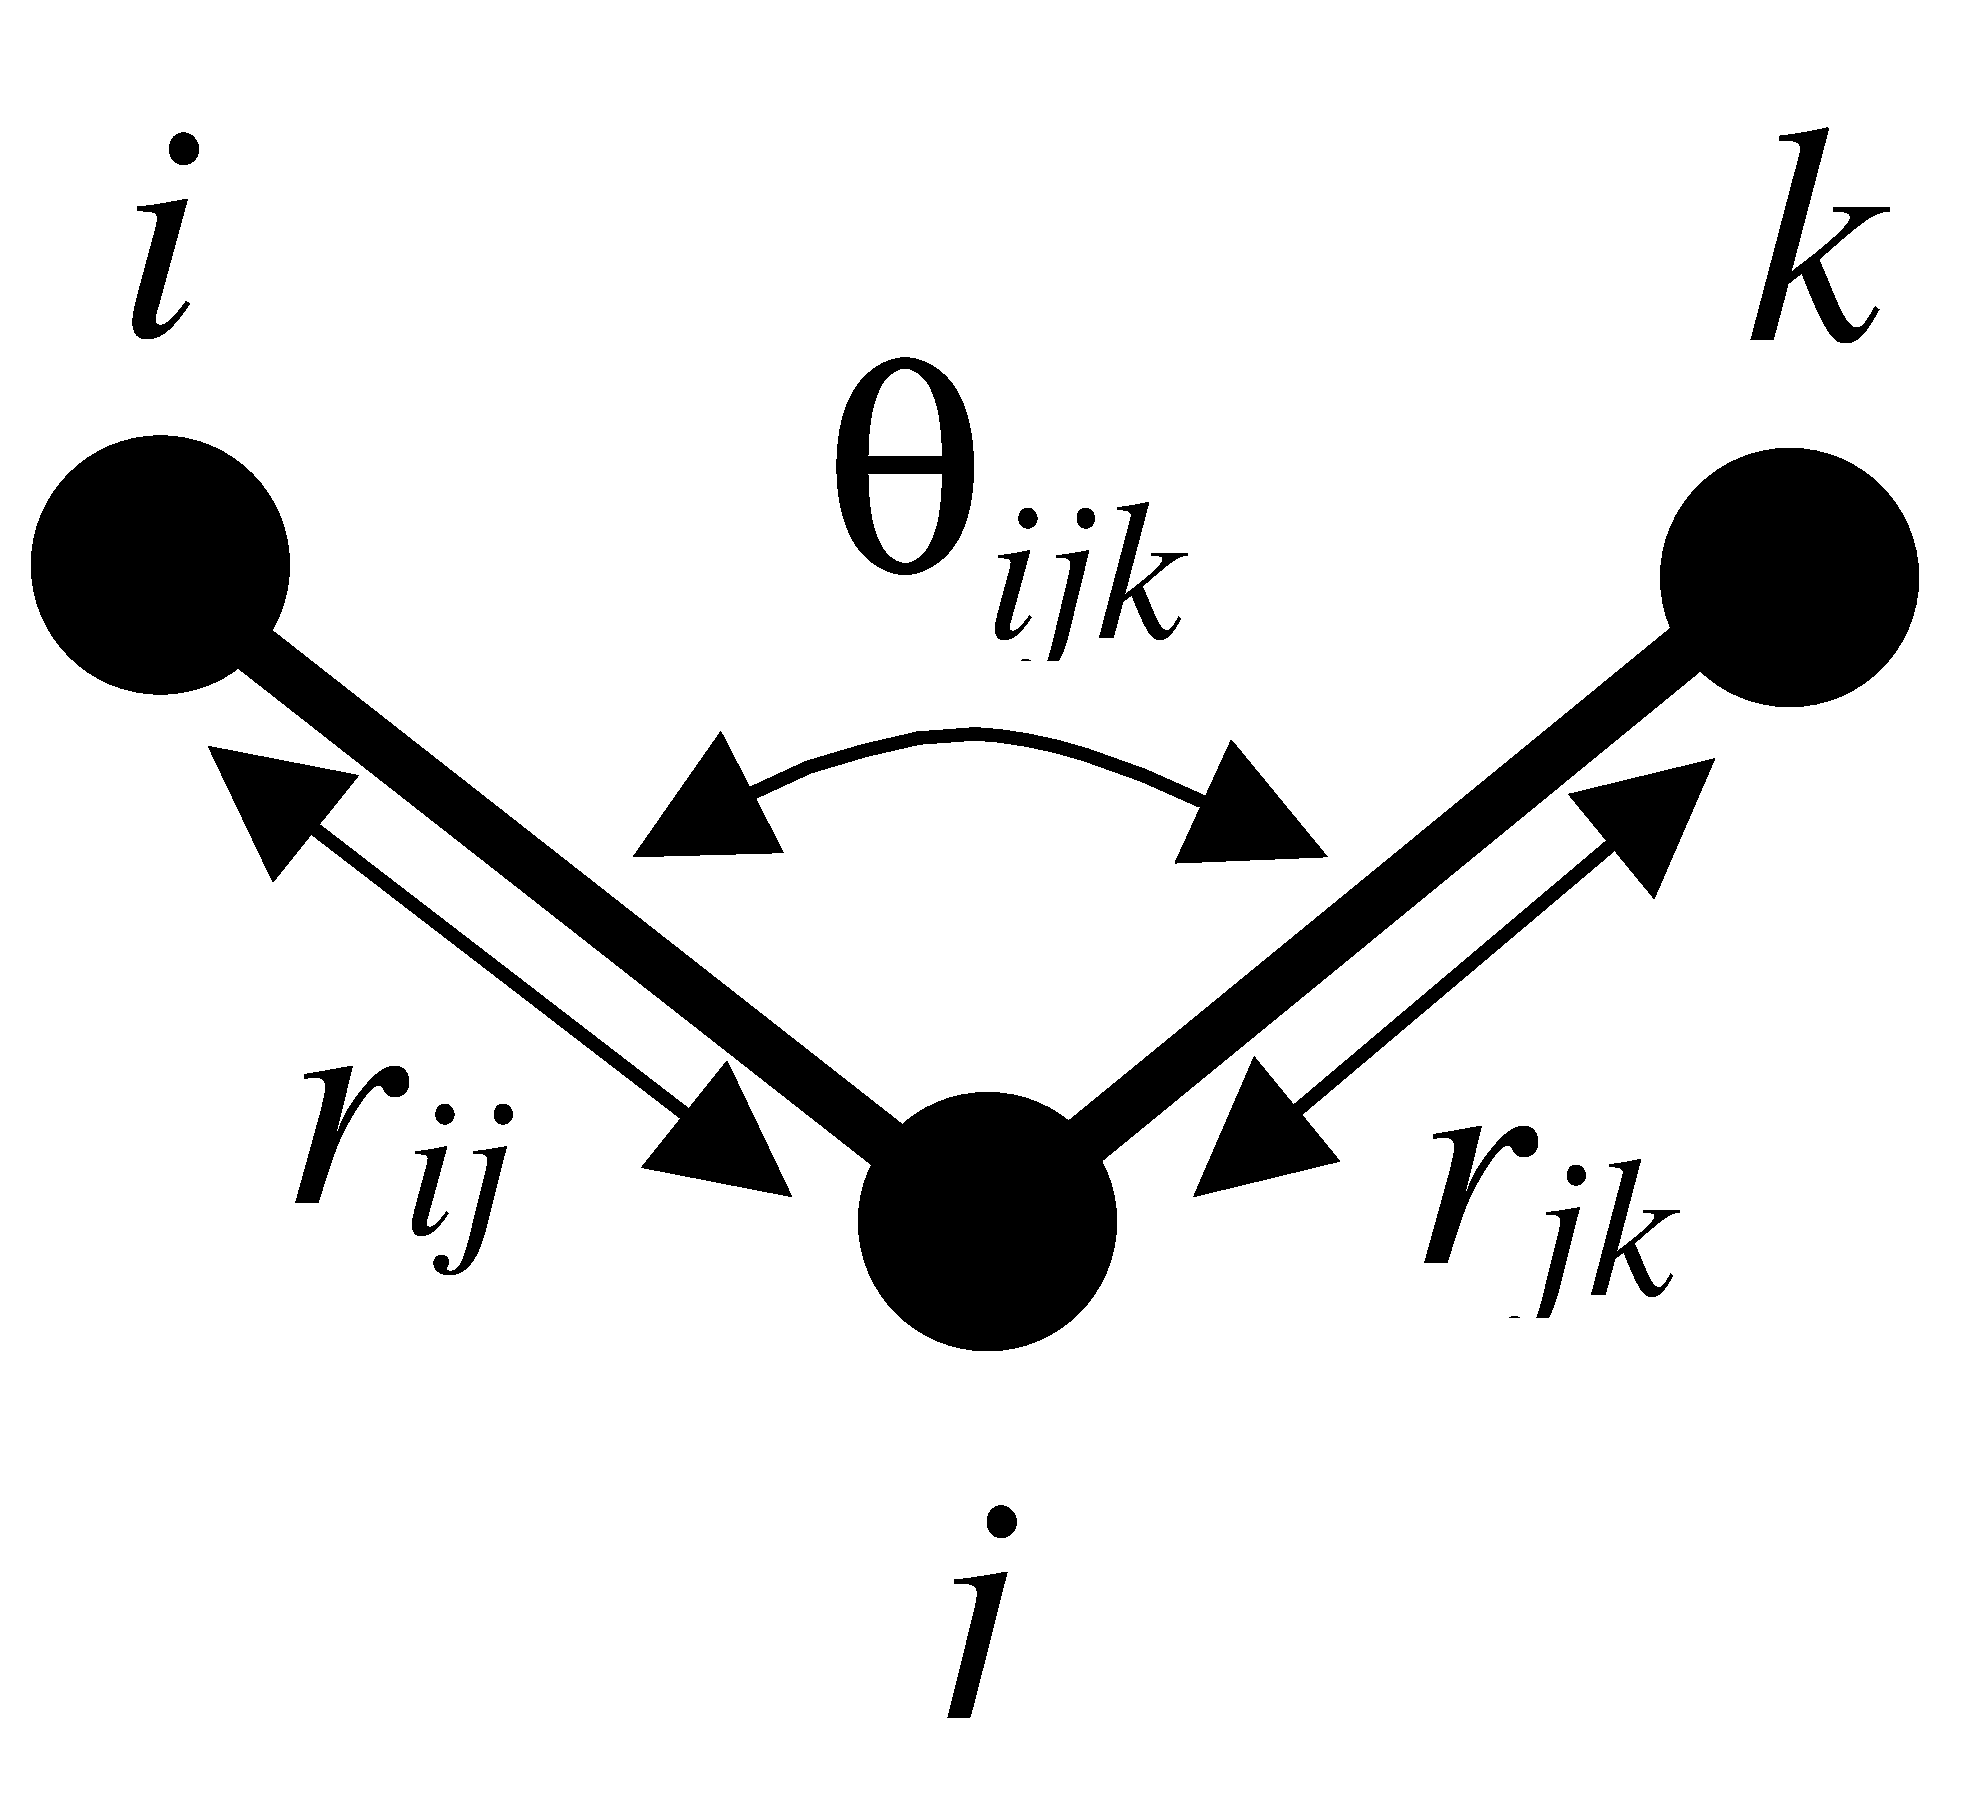
\includegraphics[%
  width=4cm,
  height=3.5cm]{mm6.eps}\begin{eqnarray}
E\left(r_{ij},r_{kj},\theta_{ijk}\right) & = & k_{ijijk}\left(r_{ij}-r_{ij}^{0}\right)\left(\theta_{ijk}-\theta_{ijk}^{0}\right)\nonumber \\
 & + & k_{kjijk}\left(r_{kj}-r_{kj}^{0}\right)\left(\theta_{ijk}-\theta_{ijk}^{0}\right)\label{eq:11}\end{eqnarray}
\end{center}

Stretching-torsion

\begin{center}\includegraphics[%
  width=6cm,
  height=3.5cm]{mm7.eps}\begin{equation}
E\left(r_{jk},\varphi_{ijkl}\right)=\frac{k_{ijkl}}{2}\left(r_{jk}-r_{jk}^{0}\right)\left[1+\cos\left(3\varphi_{ijkl}\right)\right]\label{eq:12}\end{equation}
\end{center}


\subsubsection{Core-shell interaction}

\begin{equation}
E\left(r_{i}^{c-s}\right)=\frac{k_{i}}{2}\left(r_{i}^{c-s}\right)^{2}\label{eq:15}\end{equation}



\subsection{Non-bonded interactions}


\subsubsection{Van der Waals interactions }

~~~~Buckingham\begin{equation}
E\left(r_{ij}\right)=A_{ij}\exp\left(-\frac{r_{ij}}{\rho_{ij}}\right)-\frac{C_{ij}}{r_{ij}^{6}}\label{eq:13}\end{equation}


Lennard-Jones\begin{equation}
E\left(r_{ij}\right)=\frac{A_{ij}}{r_{ij}^{12}}-\frac{C_{ij}}{r_{ij}^{6}}\label{eq:14}\end{equation}


Tabulated\begin{equation}
E\left(r_{ij}\right)=A_{ij}g\left(r_{ij}\right)+C_{ij}h\left(r_{ij}\right)\label{eq:17}\end{equation}
here $g\left(r\right)$ and $h\left(r\right)$ are user defined functions,
repulsion and dispersion terms, correspondently. That is why, $C\cdot h\left(r\right)<0$,
as rule. Functions $g\left(r\right)$ and \textit{}$h\left(r\right)$
are interpolated by cubic splines. In this case interpolating equation
looks like \begin{eqnarray}
f\left(r\right) & = & f_{i}+\delta\left\{ f_{i+1}-f_{i}-\frac{\Delta^{2}}{6}\left[2f_{i}^{\prime\prime}+f_{i+1}^{\prime\prime}\right]\right\} \nonumber \\
 & + & \delta^{3}\frac{\Delta^{2}}{6}(f_{i+1}^{\prime\prime}-f_{i}^{\prime\prime})\label{eq:18}\end{eqnarray}


and $\Delta=r_{i+1}-r_{i}$, $\delta=(r-r_{i})/\Delta$

Note that the \textit{r}-dependence is completely in $\delta$.


\subsubsection{Electrostatic interactions }

~~~~Point charge-point charge\begin{equation}
E\left(r_{ij}\right)=\frac{1}{4\pi\varepsilon_{0}}\frac{q_{i}q_{j}}{\varepsilon_{p}r_{ij}}\label{eq:21}\end{equation}


Dipole-dipole

\begin{center}\includegraphics[%
  width=5cm,
  height=4cm]{mm8.eps}\begin{equation}
E\left(R_{ij}\right)=f_{d}\frac{d_{i}d_{j}}{\varepsilon_{d}R_{ij}^{3}}\left[\cos\left(\chi_{ij}\right)-3\cos\left(\alpha_{ij}\right)\cos\left(\beta_{ij}\right)\right]\label{eq:16}\end{equation}
\end{center}

Ewald method for 3-D periodic systems\begin{eqnarray}
E & = & \frac{1}{4\pi\varepsilon_{0}}\sum_{\overrightarrow{n}}\sum_{i=1}^{N}\sum_{j=i+1}^{N}q_{i}q_{j}\frac{erfc\left(\alpha\left|\overrightarrow{r_{ij}}+\overrightarrow{n}\right|\right)}{\left|\overrightarrow{r_{ij}}+\overrightarrow{n}\right|}\nonumber \\
 & + & \frac{1}{\varepsilon_{0}V}\sum_{\overrightarrow{k}>0}\frac{\exp\left(-\frac{k^{2}}{4\alpha^{2}}\right)}{k^{2}}\left\{ \left|\sum_{i=1}^{N}q_{i}\cos\left(\overrightarrow{k}\cdot\overrightarrow{r_{i}}\right)\right|^{2}\right.\label{eq:19}\\
 & + & \left.\left|\sum_{i=1}^{N}q_{i}\sin\left(\overrightarrow{k}\cdot\overrightarrow{r_{i}}\right)\right|^{2}\right\} -\frac{1}{4\pi\varepsilon_{0}}\frac{\alpha}{\sqrt{\pi}}\sum_{i=1}^{N}q_{i}^{2}\nonumber \end{eqnarray}


Ewald method for 2-D periodic systems\begin{eqnarray}
E & = & \frac{1}{4\pi\varepsilon_{0}}\sum_{\overrightarrow{m}}\sum_{i=1}^{N}\sum_{j=i+1}^{N}q_{i}q_{j}\frac{erfc\left(\alpha\left|\overrightarrow{r_{ij}}+\overrightarrow{m}\right|\right)}{\left|\overrightarrow{r_{ij}}+\overrightarrow{m}\right|}\nonumber \\
 & + & \frac{1}{4\pi\varepsilon_{0}}\sum_{i=1}^{N}\sum_{j=i+1}^{N}\sum_{\overrightarrow{h}>0}\frac{\pi\cos\left(\overrightarrow{h}\cdot\overrightarrow{r_{ij}}\right)}{hA}\nonumber \\
 & \times & \left\{ \exp\left(hz_{ij}\right)erfc\left(\alpha z_{ij}+\frac{h}{2\alpha}\right)+\exp\left(-hz_{ij}\right)\right.\label{eq:20}\\
 & \times & \left.erfc\left(-\alpha z_{ij}+\frac{h}{2\alpha}\right)\right\} -\frac{1}{4\pi\varepsilon_{0}}\sum_{i=1}^{N}\sum_{j=i+1}^{N}q_{i}q_{j}\frac{2\pi}{A}\nonumber \\
 & \times & \left\{ z_{ij}erf\left(\alpha z_{ij}\right)+\frac{1}{\alpha\sqrt{\pi}}\exp\left[-\left(\alpha z_{ij}\right)^{2}\right]\right\} \nonumber \\
 & - & \frac{1}{4\pi\varepsilon_{0}}\frac{\alpha}{\sqrt{\pi}}\sum_{i=1}^{N}q_{i}^{2}\nonumber \end{eqnarray}



\section{Description of input file }

~~~~~To be able to run molecular mechanics job with ParaGauss
anyone has to have additional input file. It has to be named {}``\textbf{molmech.inp}''
and located inside ParaGauss input directory. This file contains information
on the type of job, the geometry of system and the force field definition
(potential parameters). To be convenient for user all input information
can be specified in arbitrary order and is non-formatted. Any number
of empty lines can be included. Comments are also available inside
input file. The important feature of a single input file is that it
can be divided in some sub-files gathered together by \textbf{include}
directives in head file. Each sub-file also can contain any number
\textbf{include} directives. Therefore a user has possibility to choose
between using the single input file or many level hierarchies of sub-files.
One of the reasons to make that choice is the size and the complexity
of molecular system under study. It is very often when molecular system
consists of many thousand atoms of different type. In this case the
single input file could be prepared, read and managed with great efforts.
A set of sub-files is a good alternative in this situation. Some files
can contain geometry of system (or its parts) or potential parameters
but others different N-body lists. 


\subsection{Common structure }

~~~~~The name {}``\textbf{molmech.inp}'' has to belong either
single input file or the main file in the set of input sub-files.
The other sub-files can have any name. Input file (or any sub-file)
consists of input data specified via NAMELIST's and special constructed
BLOCK-DATA and can include empty lines, comments and \textbf{include}
directives. Any combination of capital and small letters in keywords
is permitted (GraDienT). To comment information the symbol {}``\textbf{\#}''
is used. It can be put in any place of any input line. All information
after the comment symbol will be dropped. 

\textbf{Include} directive has to look as \textbf{\#include <file
name>}. The directive has to be placed in the beginning of separate
line otherwise it will be considered as comment. If included file
is located in the ParaGauss input directory, a user can specify in
\textbf{include} directive only its name (\textbf{\#include two\_body.list)}.
Full path is required if included file is located in any other place
than the ParaGauss input directory (\textbf{\#include} \textbf{\textit{/full\_path/}}\textbf{coordinates.dat}). 


\subsection{Input parameters }

~~~~~All input data can be specified into an input file in absolutely
arbitrary order even if they depend of each other. But for convenience
and as a good manner it is recommended to organize input file in a
definite order. 


\subsubsection{Tasks and options }

\begin{lyxlist}{00.00.0000}
\item [\textbf{Namelist}]\textbf{TOPIC}
\end{lyxlist}
\texttt{\textbf{\&topic}}

\texttt{\textbf{job\_topic = {}``name of job''}}~\\
\texttt{\textbf{/topic}} \\
\textbf{job\_topic} - character (len=100)

This namelist is used to give the name of molecular mechanics run.
Its specification is not obligatory a user can drops it in any time. 

\textit{Examples}\textit{\emph{:}}\texttt{\textit{}}~\\
\texttt{\textit{\&topic}}

\texttt{\textit{job\_topic = {}``octane'' }}~\\
\texttt{\textit{/topic}}

\begin{lyxlist}{00.00.0000}
\item [\textbf{Namelist}]\textbf{TASKS}
\end{lyxlist}
\texttt{\textbf{\&tasks}}

\texttt{\textbf{job\_tasks = {}``task1 task2 ... taskn'' }}~\\
\texttt{\textbf{/tasks }}~\\
\textbf{job\_tasks} - character(len=100) 

The namelist \textbf{TASKS} defines actions what user wants to carry
out with Molecular mecanics module. The character variable \textbf{JOB\_TASKS}
consists of some keywords managing a program run. Currently available
keywords are: \textbf{}\\
\textbf{{}``energy''} -- energy calculation; \textbf{}\\
\textbf{{}``gradients''} -- energy and gradients calculation; \textbf{}\\
\textbf{{}``optimization''} -- structural optimization of a molecular
system; \textbf{}\\
\textbf{{}``hessian'' -} calculation of second derivatives (can
conflict with \textbf{{}``optimization''} task);\textbf{}\\
\textbf{{}``to\_xyz''} -- saving molecular coordinates in XYZ format
(\textbf{molmech.xyz}); \textbf{}\\
\textbf{{}``to\_xmakemol''} -- saving molecular coordinates in format
of \textbf{Xmakemol} program;\textbf{}\\
\textbf{{}``to\_viewmol'' -} saving molecular coordinates in format
of \textbf{Viewmol} molecular visualizing software (\textbf{molmech.vm}).
This format can be used to visualize periodic and non-periodic systems;
\textbf{}\\
\textbf{{}``read\_gx''} -- reading in coordinates from a standard
\textbf{\noun{ParaGauss}} GX file, but GX file has to have name
{}``\textbf{gx.mm}'';\textbf{}\\
\textbf{{}``write\_gx''} -- writing coordinates and gradients in
GX file format. This options is launched in combination with {}``\textbf{read\_gx}''
option only; \\
\textbf{{}``to\_epe''} -- save geometry of the system (periodic
case only) in \textbf{{}``gx.cv.job\_name''} file to be used as
the unit cell in EPE calculations;\\
\textbf{{}``to\_pg\_hess''} -- save the molecular mechanics cartesian
HESSIAN in \textbf{\noun{ParaGauss}} file \textbf{{}``hesse\_cartesian.dat''}.
The last file can be used as initial HESSIAN for QM optimization (see
PG documentation). The carrent option has to be used in combination
with either \textbf{{}``optimization''} or \textbf{{}``hessian''}
keywords;\\
\textbf{{}``with\_optim''} -- using this option anyone can perform
a molecular mechanics optimization in internal coordinates. In this
case \textbf{Optimizer} of \textbf{\noun{ParaGauss}} is used. As
usual to use \textbf{Optimizer} GX file (\textbf{{}``gxfile''})
has to be exist within working directory. Please remember no {}``optimizer''
directory is created. All files are saved in the current working directory.

\textit{Examples: }\\
\texttt{\textit{\&tasks}}

\texttt{\textit{job\_tasks = {}``optimization to\_xyz'' }}~\\
\texttt{\textit{/tasks}} \textit{}\\
\textit{Optimization of molecular system has to be done and final
geometry will be saved in XYZ file {}``molmech.xyz''. }\\
\texttt{\textit{\&tasks}}

\texttt{\textit{job\_tasks = {}``gradients read\_gx write\_gx''
}}~\\
\texttt{\textit{/tasks}} \textit{}\\
\textit{The calculation of energy and gradients, the geometry has
to be taken from GX file and the result (coordinates and gradients)
will be saved in GX file also}. 

\begin{lyxlist}{00.00.0000}
\item [\textbf{Namelist}]\textbf{MAIN\_OPTIONS}
\end{lyxlist}
\texttt{\textbf{\&main\_options}}

\texttt{\textbf{coulomb ~~~~~~= .true. ~~~~~~(default
value)}}

\texttt{\textbf{van\_der\_waals = .true. ~~~~~~(default value) }}

\texttt{\textbf{rcut\_vdw ~~~~~= 10.00 ~~~~~~~(default
value) }}

\texttt{\textbf{rcut\_cs ~~~~~~= 1.0 ~~~~~~~~~(default
value) }}

\texttt{\textbf{calc\_strain ~~= .false. ~~~~~(default value) }}

\texttt{\textbf{eps ~~~~~~~~~~= 1.0 ~~~~~~~~~~(default
value)}}

\texttt{\textbf{energy\_unit ~~= {}``kJ/mol'' ~~~~~(default
value) }}

\texttt{\textbf{length\_unit ~~= {}``angstrom'' ~~~(default
value) }}

\texttt{\textbf{angle\_unit ~~~= {}``degree'' ~~~~~(default
value) }}

\texttt{\textbf{minimal\_image = .true. ~~~~~~(default value)
}}~\\
\texttt{\textbf{/main\_options }}

The current namelist defines global options acting during molecular
mechanics calculations. The namelist can be droped. 

Description of namelist data: \textbf{}\\
\textbf{Coulomb} - calculate (\textbf{true}) or not (\textbf{false})
an electrostatic interaction. \textbf{}\\
\textbf{Van\_der\_Waals} - calculate (\textbf{true}) or not (\textbf{false})
an short-range non-bonded interaction. \textbf{}\\
\textbf{Rcut\_vdw} - defines the value of cutoff radius (\textbf{�})
to calculate van der Waals interaction. \textbf{}\\
\textbf{Rcut\_cs -} define the maximal distance (\textbf{�}) to seek
core-shell pairs. \textbf{}\\
\textbf{Calc\_strain -} allow for 2- and 3-D periodic systems to calculate
first and second derivatives of energy in respect to elements of strain
tensor and, consequently, optimize lattice unit (simulation) cell
parameters. In the current version of Force Field module only periodic
electrostatic, pair van der Waals, core-shell and 3-body interactions
contribute into a strain tensor. \textbf{}\\
\textbf{Eps} - dielectric constant. \\
Next three parameters define input units to specify potential parameters.
The internal system of units of ParaGauss Force Field module is {}``\textbf{kJ/mol}''
(energy), {}``\textbf{�}'' (lengths) and {}``\textbf{�}'' (angles).
Force Field module performs all calculations using this set of units
but for user convenience there is a possibility to apply other unit
systems to specify potential parameters. User defined system of units
influences only on input data but not internal system of unit. \textbf{}\\
\textbf{Energy\_unit} - defines energy input units. Currently possible
keywords are {}``\textbf{kJ/mol}'' (default), {}``\textbf{eV}''
and {}``\textbf{kcal/mol}''. \textbf{}\\
\textbf{Length\_unit} - defines input units of length. The keywords
are {}``\textbf{angstrom}'' (default) and {}``\textbf{bohr}''.
\textbf{}\\
\textbf{Angle\_unit} - defines input angle units. Two keywords are
permitted {}``\textbf{degree}'' (default) and {}``\textbf{radian}''.
\textbf{}\\
\textbf{Minimal\_image} - defines the switch between two periodic
boundary conditions. The default value (\textbf{true}) chooses so-called
{}``minimum images'' approach. Using this approach means that only
one nearest image of each particle in the periodic boundary conditions
is considered for a pair interaction. Due to this condition, \textbf{the
cutoff radius} cannot exceed half of the simulation box (unit cell)
size. This is very useful for large systems and large simulation box.
The situation is typically true for molecules in liquids or solutions
but for solids it meets not so often. A crystal unit cell rather small
and applying {}``minimum images'' approach can produces large errors
in calculation pair non-bonded interactions. To overcome that problem
the approach considering all images of each particle satisfied the
pair potential \textbf{cutoff} condition can be used (\textbf{minimal\_image
= false}). 

\begin{lyxlist}{00.00.0000}
\item [\textbf{Namelist}]\textbf{NB\_LISTS\_OPTIONS} 
\end{lyxlist}
\texttt{\textbf{\&nb\_lists\_options }}

\texttt{\textbf{automatic\_nb\_lists = .false. (default value) }}

\texttt{\textbf{update\_nb\_list ~~~~= 1 ~~~~~~~(default
value) }}

\texttt{\textbf{exclude\_1\_2 ~~~~~~~= .true. ~(default value) }}

\texttt{\textbf{exclude\_1\_3 ~~~~~~~= .true. ~(default value) }}

\texttt{\textbf{exclude\_1\_4 ~~~~~~~= .false. (default value) }}

\texttt{\textbf{ff3\_style ~~~~~~~~~= .false. (default value)}}~\\
\texttt{\textbf{/nb\_lists\_options }}

The current namelist defines calculation of lists bonded and, consequently,
nonbonded interactions. As the previous namelist it also can be droped. 

Description of namelist data: \textbf{}\\
\textbf{Automatic\_nb\_lists -} allows automatic generation of atom
lists for covalent (bonded) and core-shell interaction basing on atomic
covalent radii (see below). Otherwise bonded lists have to be done
by hand (see bellow). In the current version an automatic generation
is possible if only 2-, 3- and core-shell bonded interactions are
specified. \textbf{}\\
\textbf{Update\_nb\_list -} this parameter is used during geometry
optimization and specifies a period of regeneration of lists of non-bonded
interactions. Currently it is not recommend to change default value. 

Next three parameters define generation of non-bonded lists for van
der Waals and electrostatic interactions. Generally atoms taking part
in bonded interactions are excluded from short- and long-range ones,
but it is not a common rule. \textbf{}\\
\textbf{Exclude\_1\_2} - exclude (or not) a calculation of non-bonded
interactions for atoms (1-2) taking part in two-body interactions.
\textbf{}\\
\textbf{Exclude\_1\_3} - exclude (or not) a calculation of non-bonded
interactions for atoms (1-2-3) taking part in three-body interactions.
\textbf{}\\
\textbf{Exclude\_1\_4} - allows excluding a calculation of non-bonded
interactions for atoms (1-4) taking part in four-body interactions.
\\
\textbf{Ff3\_style} - this option give a possibility to calculate
an electrostatic interaction between bonded atoms.

\begin{lyxlist}{00.00.0000}
\item [\textbf{Namelist}]\textbf{OPT\_OPTIONS} 
\end{lyxlist}
\texttt{\textbf{\&opt\_options }}

\texttt{\textbf{n\_ierations ~~~~~~~= 1000 ~~~~~~~(default
value) }}

\texttt{\textbf{method ~~~~~~~~~~~~= {}``newton'' ~~~(default
value) }}

\texttt{\textbf{gnorm ~~~~~~~~~~~~~= 1.0e-5 ~~~~~(default
value) }}

\texttt{\textbf{gmax ~~~~~~~~~~~~~~= 1.0e-4 ~~~~~(default
value)}}

\texttt{\textbf{rnorm ~~~~~~~~~~~~~= 1.0e-5 ~~~~~(default
value) }}

\texttt{\textbf{rmax ~~~~~~~~~~~~~~= 1.0e-4 ~~~~~(default
value) }}

\texttt{\textbf{hess\_update\_cycles = 10 ~~~~~~~~~(default
value) }}

\texttt{\textbf{max\_step ~~~~~~~~~~= 1.0 ~~~~~~~~(default
value) }}

\texttt{\textbf{ls\_method ~~~~~~~~~= {}``3-parab'' ~~(default
value) }}~\\
\texttt{\textbf{/opt\_options }}

The namelist \textbf{OPT\_OPTIONS} controls geometry optimization
of the molecular system under study. It can be dropped if the default
values of namelist parameters are used. 

Namelist description: \textbf{}\\
\textbf{N\_iterations} - defines the total number of iterations steps.
There is not an up limit for this parameter. \textbf{}\\
\textbf{Method} - this parameter in a future will allow to choose
method of optimization. Currently only Newton-Raphson method ({}``\textbf{newton}'')
was implemented. Please do not modify this parameter. The program
will obstruct any attempts to do it. 

The next four parameters are the conditions of a geometry optimization
convergence. The optimization will be stoped if all four parameters
are not exceeding the predefined values. \textbf{}\\
\textbf{Gnorm} - the maximal gradient norm. \textbf{}\\
\textbf{Gmax} - the maximal absolute value of any gradient component.
\textbf{}\\
\textbf{Rnorm} - the maximal norm geometry-updating step. \textbf{}\\
\textbf{Rmax} - the maximal absolute value of geometry-updating step
along any Cartesian coordinate. \textbf{}\\
\textbf{Hess\_update\_cycles -} number of geometry optimization cycles
after that the Hessian has to be recalculated. \textbf{}\\
\textbf{Max\_step -} controls a relative value of calculated geometry
step. \textbf{}\\
\textbf{Ls\_method -} defines choosing between different algorithms
of a line search method. Two keywords are allowed. The keyword \textbf{{}``3-parab''}
chooses a line search algorithm basing on calculating a cubic parabola.
The other keyword \textbf{{}``step''} switches on a algorithm of
{}``half geometry step''. 

\begin{lyxlist}{00.00.0000}
\item [\textbf{Namelist}]\textbf{HESS\_OPTIONS} 
\end{lyxlist}
\texttt{\textbf{\&hess\_options }}

\texttt{\textbf{hess\_type ~~= {}``unit'' ~~(default value) }}

\texttt{\textbf{weight\_hess = 1.0 ~~~~~(default value) }}~\\
\texttt{\textbf{/hess\_options}}

The namelist \textbf{HESS\_OPTIONS} is used together with the namelist
\textbf{OPT\_OPTIONS}. It also can be dropped if default parameters
are used. 

Description of the namelist parameters:\textbf{}\\
\textbf{Hess\_type} - defines the type of an initial hessian to perform
the Newton-Raphson optimization. Three keywords can be used: {}``\textbf{UNIT}''
- the initial hessian is a diagonal matrix, {}``\textbf{NUMERICAL}''
- the hessian will be calculated by numerical differentiation of gradients
and {}``\textbf{ANALYTICAL}'' - the analytically calculated hessian
will be used. If analytical second derivatives are available for all
used interactions applying analytical hessian is preferable. \textbf{}\\
\textbf{Weight\_hess} - this parameter is important only if the previous
parameter is {}``\textbf{UNIT}''. It allows to reduce values of
the hessian diagonal matrix. 


\subsubsection{Definition of molecular system }

~~~~To be able to apply periodic boundary conditions (3-D or 2-D)
anyone has to define three (two) vectors of simulation (unit) cell,
or six (three) lattice (slab) parameters (see figure \textbf{)}

\begin{lyxlist}{00.00.0000}
\item [\textbf{Namelists}]\textbf{VECTORS and VECTORS\_SLAB} 
\end{lyxlist}
\texttt{\textbf{\&vectors }}

\texttt{\textbf{vector1 = x1, y1, z1 }}

\texttt{\textbf{vector2 = x2, y2, z2 }}

\texttt{\textbf{vector3 = x3, y3, z3 }}~\\
\texttt{\textbf{/vectors}} \\
and \textbf{}\\
\texttt{\textbf{\&vectors\_slab}}

\texttt{\textbf{vector1 = x1, y1 }}

\texttt{\textbf{vector2 = x2, y2 }}~\\
\texttt{\textbf{/vectors\_slab}} 

Namelists \textbf{VECTORS} and \textbf{VECTORS\_SLAB} define 3- or
2-D unit cells by means unit cell vectors. For 2-D case (slab) vectors
define periodicity in two directions perpendicular to Z axis. 

\begin{lyxlist}{00.00.0000}
\item [\textbf{Namelists}]\textbf{CELL and CELL\_SLAB} 
\end{lyxlist}
\texttt{\textbf{\&cell}}

\texttt{\textbf{a ~~~~= ??? }}

\texttt{\textbf{b ~~~~= ???}}

\texttt{\textbf{c ~~~~= ??? }}

\texttt{\textbf{alpha = ??? }}

\texttt{\textbf{beta ~= ??? }}

\texttt{\textbf{gamma = ??? }}~\\
\texttt{\textbf{/cell}} \\
and \textbf{}\\
\texttt{\textbf{\&cell\_slab }}

\texttt{\textbf{a ~~~~= ??? }}

\texttt{\textbf{b ~~~~= ??? }}

\texttt{\textbf{alpha = ??? }}~\\
\texttt{\textbf{/cell\_slab }}

Alternative way to define simulation (unit) cell is to specify cell
parameters: lengths of cell sides and angles between them.

Namelist description: \textbf{}\\
\textbf{A, b, c -} lengths of unit cell sides (�)\textbf{,}\\
\textbf{Alpha, beta, gamma -} unit cell angles (�) 

\begin{lyxlist}{00.00.0000}
\item [\textbf{Blocks}]\textbf{of data CARTESIAN\_COOR and FRACTIONAL\_COOR}
\end{lyxlist}
~~~~Blocks of data were specially derived to specify into input
file more or less uniform data, which are not suitable to be inputted
by namelists. In current version of Molecular Mechanics module blocks
of data are exploited to define molecular coordinates and N-body lists
of bonded interactions. In some details block of data looks like standard
Fortran namelist but it is not a namelist. All data inside block of
data are not formatted. \textbf{}\\
\texttt{\textbf{\&cartesian\_coor }}~\\
\texttt{\textbf{atnam1 cs xcoor1 ycoor1 zcoor1 }}~\\
\texttt{\textbf{atnam2 cs xcoor2 ycoor2 zcoor2 }}~\\
\texttt{\textbf{..............................}}~\\
\texttt{\textbf{atnamN cs xcoorN ycoorN zcoorN }}~\\
\texttt{\textbf{/cartesian\_coor}} \\
or \textbf{}\\
\texttt{\textbf{\&fractional\_coor }}~\\
\texttt{\textbf{atnam1 cs xfrac1 yfrac1 zfrac1}}~\\
\texttt{\textbf{atnam2 cs xfrac2 yfrac2 zfrac2 }}~\\
\texttt{\textbf{..............................}}~\\
\texttt{\textbf{atnamN cs xfracN yfracN zfracN }}~\\
\texttt{\textbf{/fractional\_coor}} \\
or \textbf{}\\
\texttt{\textbf{\&fractional\_coor (slab case) }}~\\
\texttt{\textbf{atnam1 cs xfrac1 yfrac1 zcoor1 }}~\\
\texttt{\textbf{atnam2 cs xfrac2 yfrac2 zcoor2 }}~\\
\texttt{\textbf{..............................}}~\\
\texttt{\textbf{atnamN cs xfracN yfracN zcoorN }}~\\
\texttt{\textbf{/fractional\_coor}}

Block of data \textbf{CARTESIAN\_COOR} defines the molecular geometry
in Cartesian coordinates and can be applied to periodical and non-periodical
systems. \textbf{FRACTIONAL\_COOR} block of data is used to specify
atom coordinates of periodic systems in internal form. The special
case is 2-D system. For such system \textbf{FRACTIONAL\_COOR} block
of data contains only X and Y coordinates in internal form. Z coordinates
is in Cartesian one.

Description of parameters: \textbf{}\\
\textbf{Atnam} - unique name of atom or other species. The length
of atom name cannot exceed six symbols (letters and digits), for example
: H1, Cu\_2, AG30. \textbf{}\\
\textbf{Cs} - serves to present atoms as consisting of core (\textbf{{}``c''})
and shell (\textbf{{}``s''}) (core-shell polarization model). In
rigid model all atoms are considered as core (\textbf{{}``c''}).
\textbf{Cs} parameter can be dropped if atom (species) is {}``core''.
\textbf{}\\
\textbf{Xcoor}, \textbf{ycoor} and \textbf{zcoor} - X, Y and Z cartesian
coordinates of each specified atom (species) \textbf{}\\
\textbf{Xfrac}, \textbf{yfrac} and \textbf{zfrac} - X, Y and Z fractional
(internal) coordinates of atoms (species) 

\textit{Example}\textit{\emph{:}} \emph{}\\
\texttt{\textit{\&cartesian\_coor }}~\\
\texttt{\textit{C ~c -0.231579 -0.370841 -0.037475 }}~\\
\texttt{\textit{C ~c ~0.229441 ~0.373160 ~1.224850 }}~\\
\texttt{\textit{O ~c ~0.868228 -0.551628 ~2.114423 }}~\\
\texttt{\textit{H0 c ~0.619613 -0.833754 -0.565710 }}~\\
\texttt{\textit{H0 c -0.709445 ~0.352087 -0.754607 }}~\\
\texttt{\textit{H0 c -0.976393 -1.144198 ~0.191635 }}~\\
\texttt{\textit{H2 c -0.628785 ~0.860022 ~1.736350 }}~\\
\texttt{\textit{H2 c ~0.952253 ~1.174538 ~0.962081 }}~\\
\texttt{\textit{H1 c ~0.204846 -1.119563 ~2.483509 }}~\\
\texttt{\textit{/cartesian\_coor }}

\begin{lyxlist}{00.00.0000}
\item [\textbf{Namelist}]\textbf{SPECIES}
\end{lyxlist}
\texttt{\textbf{\&species }}

\texttt{\textbf{name ~~~~~~~= {}``atname'' }}

\texttt{\textbf{main\_name ~~= {}``in'' }}

\texttt{\textbf{r\_coval ~~~~= 0.0 (default value) }}

\texttt{\textbf{charge ~~~~~= 0.0 (default value) }}

\texttt{\textbf{vdw\_red\_fac = 1.0 (default value) }}~\\
\texttt{\textbf{/species}} 

The namelist \textbf{SPECIES} defines (if necessary) properties of
atoms (species) forming the molecular system. These namelists can
be specified for some atoms or drooped at all but the total number
of namelists specified cannot exceed the number of different atom
(species) types into the molecular system. 

Description of namelist data: \textbf{}\\
\textbf{Name} - the name of atom type. This name must coincide with
one of the atom names in \textbf{CARTESIAN\_COOR} (\textbf{FRACTIONAL\_COOR})
block of data.\textbf{}\\
\textbf{Main\_name} - serves to tie atoms in the molecular system
with predefined properties (in current version only covalent radii
are available). If used, \textbf{main\_name} has to be equal to the
one of internal atom names (see Appendix 1). \textbf{}\\
\textbf{R\_coval} - allows to define a covalent radius for specific
atom type (in \textbf{�}). If \textbf{r\_coval} is equal zero and
\textbf{main\_name} parameter was specified the predefined covalent
radius is used. \textbf{}\\
\textbf{Charge} - this parameter is used to define the charge of atoms
\textbf{}\\
\textbf{Vdw\_red\_fac} - the appearance of this parameter is due to
MM3 force field implementation. This force field considers hydrogen
atom forming \textbf{H-X} bond as located closer to atom X to calculate
van der Waals interaction. For \textbf{H} atom \textbf{vdw\_red\_fac}
is equal 0.923. It means during calculation of van der Waals interaction
coordinates of hydrogen atoms are recalculated to shorten \textbf{H-X}
bond. For most types of atom in MM3 force field and for other force
fields the default value (1.0) is applied. 


\subsubsection{Force Field definition }

\begin{lyxlist}{00.00.0000}
\item [\textbf{Namelist}]\textbf{POTENTIAL} 
\end{lyxlist}
\texttt{\textbf{\&potential }}

\texttt{\textbf{pot\_name ~~~~= {}``name'' }}

\texttt{\textbf{atom\_name ~~~= {}``atnm1'', {}``atnm2'', {}``atnm3'',
... }}

\texttt{\textbf{ff\_parameter = ffp1, ffp2, ffp3, ... }}

\texttt{\textbf{read\_data ~~~= {}``no'' (default value) }}~\\
\texttt{\textbf{/potential }}

This namelist is used to define potential functions (force field used).
The same namelist is applied to specify different potential functions. 

Description of namelist options: \textbf{}\\
\textbf{Pot\_name} - name of potential. \textbf{}\\
\textbf{Atom\_name} - list of names of atoms participated in the interaction.
\textbf{}\\
\textbf{Ff\_parameter} - list of potential parameters. \textbf{}\\
\textbf{Read\_data} - this parameter in the current version is used
only in frameworks of van der Waals interactions and specifies name
of file that contains data (in tabulate form) of a user defined potential.
To define name of data file the same rules as for include files act
here. If the file is located in the input directory only name of file
can be used, otherwise full path has to be applied. 

\textit{Examples:}\\
\textit{a) Stretching potentials}\texttt{\textit{}}~\\
\texttt{\textit{\&potential~~~~~}}\textit{(harmonic)}

\texttt{\textit{pot\_name = ''harm\_str'' }}

\texttt{\textit{atom\_name = {}``at$_{i}$'', {}``at$_{j}$''}}

\texttt{\textit{ff\_parameter = k2$_{ij}$, r$_{ij}^{0}$ }}~\\
\texttt{\textit{/potential }}~\\
\texttt{\textit{\&potential ~~~~~}}\textit{(quartic)}

\texttt{\textit{pot\_name = {}``quart\_str''}}

\texttt{\textit{atom\_name = {}``at$_{i}$'', {}``at$_{j}$'' }}

\texttt{\textit{ff\_parameter = k2$_{ij}$, k3$_{ij}$, k4$_{ij}$,
r$_{ij}^{0}$ }}~\\
\texttt{\textit{/potential }}~\\
 \texttt{\textit{\&potential ~~~~~}}\textit{(morse)}

\texttt{\textit{pot\_name = {}``morze''}}

\texttt{\textit{atom\_name = {}``at$_{i}$i'', {}``at$_{j}$j'' }}

\texttt{\textit{ff\_parameter = D$_{ij}$, A$_{ij}$, r$_{ij}^{0}$
}}~\\
\texttt{\textit{/potential }}~\\
\texttt{\textit{\&potential~~~~~}}\textit{(buckingham)}

\texttt{\textit{pot\_name = {}``bck\_short''}}

\texttt{\textit{atom\_name = {}``at$_{i}$'', {}``at$_{j}$'',
{}``at$_{k}$''}}

\texttt{\textit{ff\_parameter = A$_{ij}$, $\rho_{ij}$, C$_{ij}$
}}~\\
\texttt{\textit{/potential}}%
\footnote{Including Buchingham potential ({}``bsk\_short'') in a set of bonded
interactions has been inspired by developing alumino-silicate core-shell
force field based on atomic potential derived charges ({}``FF3'')
to describe as rule interactions between oxygen atoms forming TO$_{4}$
tetrahedra (here, T is either Si or Al atom). Interaction between
two \emph{i} and \emph{j} oxygen atoms included in the same TO$_{4}$
group can depend on the type of T atom. That is why, {}``\textbf{bsk\_short}''
depends on three atoms (\emph{i, j} and \emph{k}). \emph{k} atom is
common for both \emph{i} and \emph{j} atoms (bonded). 

The potential can also be applied to describe interaction between
atoms which have no a common atom. In this case third atom has to
be named {}``\textbf{NN}''%
} \texttt{\textit{}}\\
\textit{b) Bending potentials} \textit{}\\
\texttt{\textit{\&potential ~~~~~}}\textit{(harmonic)}

\texttt{\textit{pot\_name = {}``harm\_bnd'' }}

\texttt{\textit{atom\_name = {}``at$_{i}$'', {}``at$_{i}$'',
{}``at$_{k}$'' }}

\texttt{\textit{ff\_parameter = k2$_{ijk}$, $\theta$$_{ijk}^{0}$
}}~\\
\texttt{\textit{/potential }}~\\
\texttt{\textit{\&potential~~~~~}}\textit{(quartic)}

\texttt{\textit{pot\_name = {}``quart\_bnd'' }}

\texttt{\textit{atom\_name = {}``at$_{i}$'', {}``at$_{j}$'',
{}``at$_{k}$'' }}

\texttt{\textit{ff\_parameter = k2$_{ijk}$, k3$_{ijk}$, k4$_{ijk}$,
$\theta$$_{ijk}^{0}$}}~\\
\texttt{\textit{/potential }}~\\
\texttt{\textit{\&potential~~~~~}}\textit{(six)}

\texttt{\textit{pot\_name = {}``six\_bnd'' }}

\texttt{\textit{atom\_name = {}``at$_{i}$'', {}``at$_{j}$'',
{}``at$_{k}$'' }}

\texttt{\textit{ff\_parameter = k2$_{ijk}$, k3$_{ijk}$, k4$_{ijk}$,
k5$_{ijk}$, k6$_{ijk}$, $\theta$$_{ijk}^{0}$}}~\\
\texttt{\textit{/potential}} \\
\textit{c) Torsion potentials} \\
\texttt{\textit{\&potential~~~~~}}\textit{(harmonic)}

\texttt{\textit{pot\_name = {}``harm\_trs'' }}

\texttt{\textit{atom\_name = {}``at$_{i}$'', {}``at$_{j}$'',
{}``at$_{k}$'', {}``at$_{l}$'' }}

\texttt{\textit{ff\_parameter = k2$_{ijkl}$, $\varphi_{ijkl}^{0}$
}}~\\
\texttt{\textit{/parameter }}~\\
\texttt{\textit{\&potential~~~~~}}\textit{(triple cosine)}

\texttt{\textit{pot\_name = {}``tripl\_cos'' }}

\texttt{\textit{atom\_name = {}``at$_{i}$'', {}``at$_{j}$'',
{}``at$_{k}$'', {}``at$_{l}$'' }}

\texttt{\textit{ff\_parameter = k1$_{ijkl}$, k2$_{ijkl}$, k3$_{ijkl}$
}}~\\
\texttt{\textit{/potential}} \\
\textit{d) Cross terms} \\
\texttt{\textit{\&potential~~~~~}}\textit{(stretching-stretching)}

\texttt{\textit{pot\_name = {}``str\_str'' }}

\texttt{\textit{atom\_name = {}``at$_{i}$'', {}``at$_{j}$'',
{}``atm$_{k}$'' }}

\texttt{\textit{ff\_parameter = k$_{ijk}$, r$_{ij}^{0}$, r$_{jk}^{0}$
}}~\\
\texttt{\textit{/potential}}~\\
\texttt{\textit{\&potential~~~~~}}\textit{(bending-bending)}

\texttt{\textit{pot\_name = {}``bnd\_bnd'' }}

\texttt{\textit{atom\_name = {}``at$_{i}$'', {}``at$_{k}$'',
{}``at$_{j}$'', {}``at$_{l}$'', {}``at$_{m}$'' }}

\texttt{\textit{ff\_parameter = k$_{ikjlm}$, $\theta_{ijk}^{0}$,
$\theta_{ljm}^{0}$}}~\\
\texttt{\textit{/potential }}~\\
\texttt{\textit{\&potential~~~~~}}\textit{(stretching-bending)}

\texttt{\textit{pot\_name = {}``str\_bnd''}}

\texttt{\textit{atom\_name = {}``at$_{i}$'', {}``at$_{j}$'',
{}``at$_{k}$'' }}

\texttt{\textit{ff\_parameter = k$_{ijk}$, r$_{ij}^{0}$, r$_{jk}^{0}$,
$\theta_{ijk}^{0}$}}~\\
\texttt{\textit{/potential }}~\\
\texttt{\textit{\&potential~~~~~}}\textit{(stretching-torsion)}

\texttt{\textit{pot\_name =''str\_trs''}}

\texttt{\textit{atom\_name = {}``at$_{i}$'', {}``at$_{j}$'',
{}``at$_{k}$'', {}``at$_{l}$'' }}

\texttt{\textit{ff\_parameter = k$_{ijkl}$, r$_{jk}^{0}$}}~\\
\texttt{\textit{/potential}}\\
\texttt{\textit{\&potential~~~~~}}\textit{(core-shell)}

\texttt{\textit{pot\_name =''core\_shell''}}

\texttt{\textit{atom\_name = {}``at$_{i}$ c'', {}``at$_{i}$ s'' }}

\texttt{\textit{ff\_parameter = k$_{i}$}}~\\
\texttt{\textit{/potentia}}\\
\textit{e) Van der Waals potentials} \\
\texttt{\textit{\&potential~~~~~}}\textit{(buckingham)}

\texttt{\textit{pot\_name = {}``buck''}}

\texttt{\textit{atom\_name = {}``at$_{i}$'', {}``at$_{j}$'' }}

\texttt{\textit{ff\_parameter = A$_{ij}$, $\rho_{ij}$, C$_{ij}$
}}~\\
\texttt{\textit{/potential }}~\\
\texttt{\textit{\&potential~~~~~}}\textit{(lennard\_jones)}

\texttt{\textit{pot\_name = {}``l\_j''}}

\texttt{\textit{atom\_name = {}``at$_{i}$'', {}``at$_{j}$'' }}

\texttt{\textit{ff\_parameter = A$_{ij}$, C$_{ij}$}}~\\
\texttt{\textit{/potential}}~\\
\texttt{\textit{\&potential~~~~~}}\textit{(tabulated)}

\texttt{\textit{pot\_name = {}``user'' }}

\texttt{\textit{atom\_name = {}``at$_{i}$'', {}``at$_{j}$''}}

\texttt{\textit{ff\_parameter = A$_{ij}$, C$_{ij}$ }}

\texttt{\textit{read\_data = {}``file\_name'' }}~\\
\texttt{\textit{/potential}} \\
The tast example describe specification of currently coded short range
potentials (bonded and non-bonded). See functional forms of potentials
in the beginning of the document for correct inputting force field
parameters. The description of file containing data of user-defined
potential is in Appendix 2. 

\begin{lyxlist}{00.00.0000}
\item [\textbf{Namelist}]\textbf{ELECTROSTATIC}
\end{lyxlist}
~~~~The namelist \textbf{ELECTROSTATIC} manages choosing type
of Coulomb interactions and consists only of single parameter. Default
option is the direct Coulomb summation of point charges, no any cutoff
distances are applied. The charges has to be defined by namelist \textbf{SPECIES}
for each atom type. The name list \textbf{COULOMB} can be dropped
if the default variant is used.\textbf{}\\
\texttt{\textbf{\&electrostatic}}

\texttt{\textbf{coulomb\_type = {}``direct'' (default value) }}~\\
\texttt{\textbf{/electrostatic}}

Description of namelist: \textbf{}\\
\textbf{Coulomb\_type} - the parameter defines the choice between
point charge - point charge and dipole - dipole type of interactions.
Two meanings are permitted : {}``\textbf{direct}'' - interaction
of point charges and {}``\textbf{dipole-dipole}'' - interaction
of bond dipoles. The first value is default option. If simulated system
is periodic, automatically \textbf{Ewald} method will be chosen.

\begin{lyxlist}{00.00.0000}
\item [\textbf{Namelist}]\textbf{BOND\_DIPOLE} 
\end{lyxlist}
\texttt{\textbf{\&bond\_dipole }}

\texttt{\textbf{atom\_name = {}``atnm1'', {}``atnm2'' }}

\texttt{\textbf{dip\_mom ~~= zero (default value)}}~\\
\texttt{\textbf{/bond\_dipole}}

The namelist \textbf{BOND\_DIPOLE} has to be specified if {}``\textbf{dipole-dipole}''
type of electrostatic interaction was chosen. 

Namelist description: \textbf{}\\
\textbf{Atom\_name} - defines the pair of atoms forming a bond dipole.
Bond dipoles are defined automatically for pair of atoms having chemical
bond. For this aim the atom covalent radii are applied. That is why
the user has either to specify the correct radii by \textbf{SPECIES}
namelist or to use predefined values. In the last case either the
atom name or \textbf{main\_name} parameter into \textbf{SPECIES} namelist
has to be equal the internal atom name.\textbf{}\\
\textbf{Dip\_mom} - this is the value of bond dipole moment (Debay) 


\subsubsection{Blocks of data forming N-body lists for covalent interactions. }

~~~~Covalent interactions are calculated basing on so-called {}``\textbf{N-body}''
lists. As rule for the most part of molecular mechanics (dynamics)
programs those lists have to be prepared by hands (for large molecules
like proteins \textbf{N-body} lists can be extracted from \textbf{PDB}
files). The number and types of \textbf{N-body} lists have to correspond
to the set of used covalent potentials. \textbf{N-body lists} blocks
of data are common for different potentials of the same type and contain
lists of atoms numbers taking part in covalent interaction: \textbf{}\\
\texttt{\textbf{\&two\_body\_list }}

\texttt{\textbf{i ~j }}

\texttt{\textbf{.... }}~\\
\texttt{\textbf{/two\_body\_list}}\textbf{}\\
\textbf{Two\_body\_list} defines the list of atom pairs taking part
in \textbf{stretching} interactions. \textbf{}\\
\texttt{\textbf{\&three\_body\_list }}

\texttt{\textbf{i ~j ~k }}

\texttt{\textbf{....... }}~\\
\texttt{\textbf{/three\_body\_list}} \textbf{}\\
\textbf{Three\_body\_list} forms the atom list for \textbf{bending}
potentials. \textbf{}\\
\texttt{\textbf{\&four\_body\_list }}

\texttt{\textbf{i ~j ~k ~l }}

\texttt{\textbf{.......... }}~\\
\texttt{\textbf{/four\_body\_list}}\textbf{}\\
\textbf{Four\_body\_list} serves to define atoms taking part in \textbf{torsion}
interactions. \textbf{}\\
\texttt{\textbf{\&str\_str\_list }}

\texttt{\textbf{i ~j ~k }}

\texttt{\textbf{....... }}~\\
\texttt{\textbf{/str\_str\_list}} \textbf{}\\
\textbf{Str\_str\_list} defines the atom list for \textbf{stretching-stretching}
interactions. \textbf{}\\
\texttt{\textbf{\&bnd\_bnd\_list }}

\texttt{\textbf{i ~k ~j ~l ~m }}

\texttt{\textbf{............. }}~\\
\texttt{\textbf{/bnd\_bnd\_list}}\\
\textbf{Bnd\_bnd\_list} defines the atom list for \textbf{bending-bending}
potentials. \textbf{}\\
\texttt{\textbf{\&str\_bnd\_list}}

\texttt{\textbf{i ~j ~k }}

\texttt{\textbf{.......}}~\\
\texttt{\textbf{/str\_bnd\_list}}\textbf{}\\
\textbf{Str\_bnd\_list} forms the \textbf{stretching-bending} potential
atom list.\textbf{}\\
\texttt{\textbf{\&str\_trs\_list}}

\texttt{\textbf{i ~j ~k ~l }}

\texttt{\textbf{.......... }}~\\
\texttt{\textbf{/str\_trs\_list}} \textbf{}\\
\textbf{Str\_trs\_list} defines the \textbf{stretching-torsion} potential
atom list. 

There is alternative possibility to define \textbf{N-body lists}.
If only 2-, 3-body and core-shell types of bonded interactions are
used to model a system under study a user can choose automatic definition
of bonded lists (\textbf{automatic\_nb\_lists} = \textbf{TRUE}). Please
remember, automatic procedure is based on correct covalent radii of
atoms, which have to be defined in \textbf{SPECIES} namelists. 

\textit{Example:} 

\emph{To avoid mistakes and misunderstanding the example of} \textbf{\emph{N-body
lists}} \emph{blocks of data are exhibited basing on C2H5OH molecules.}

\begin{center}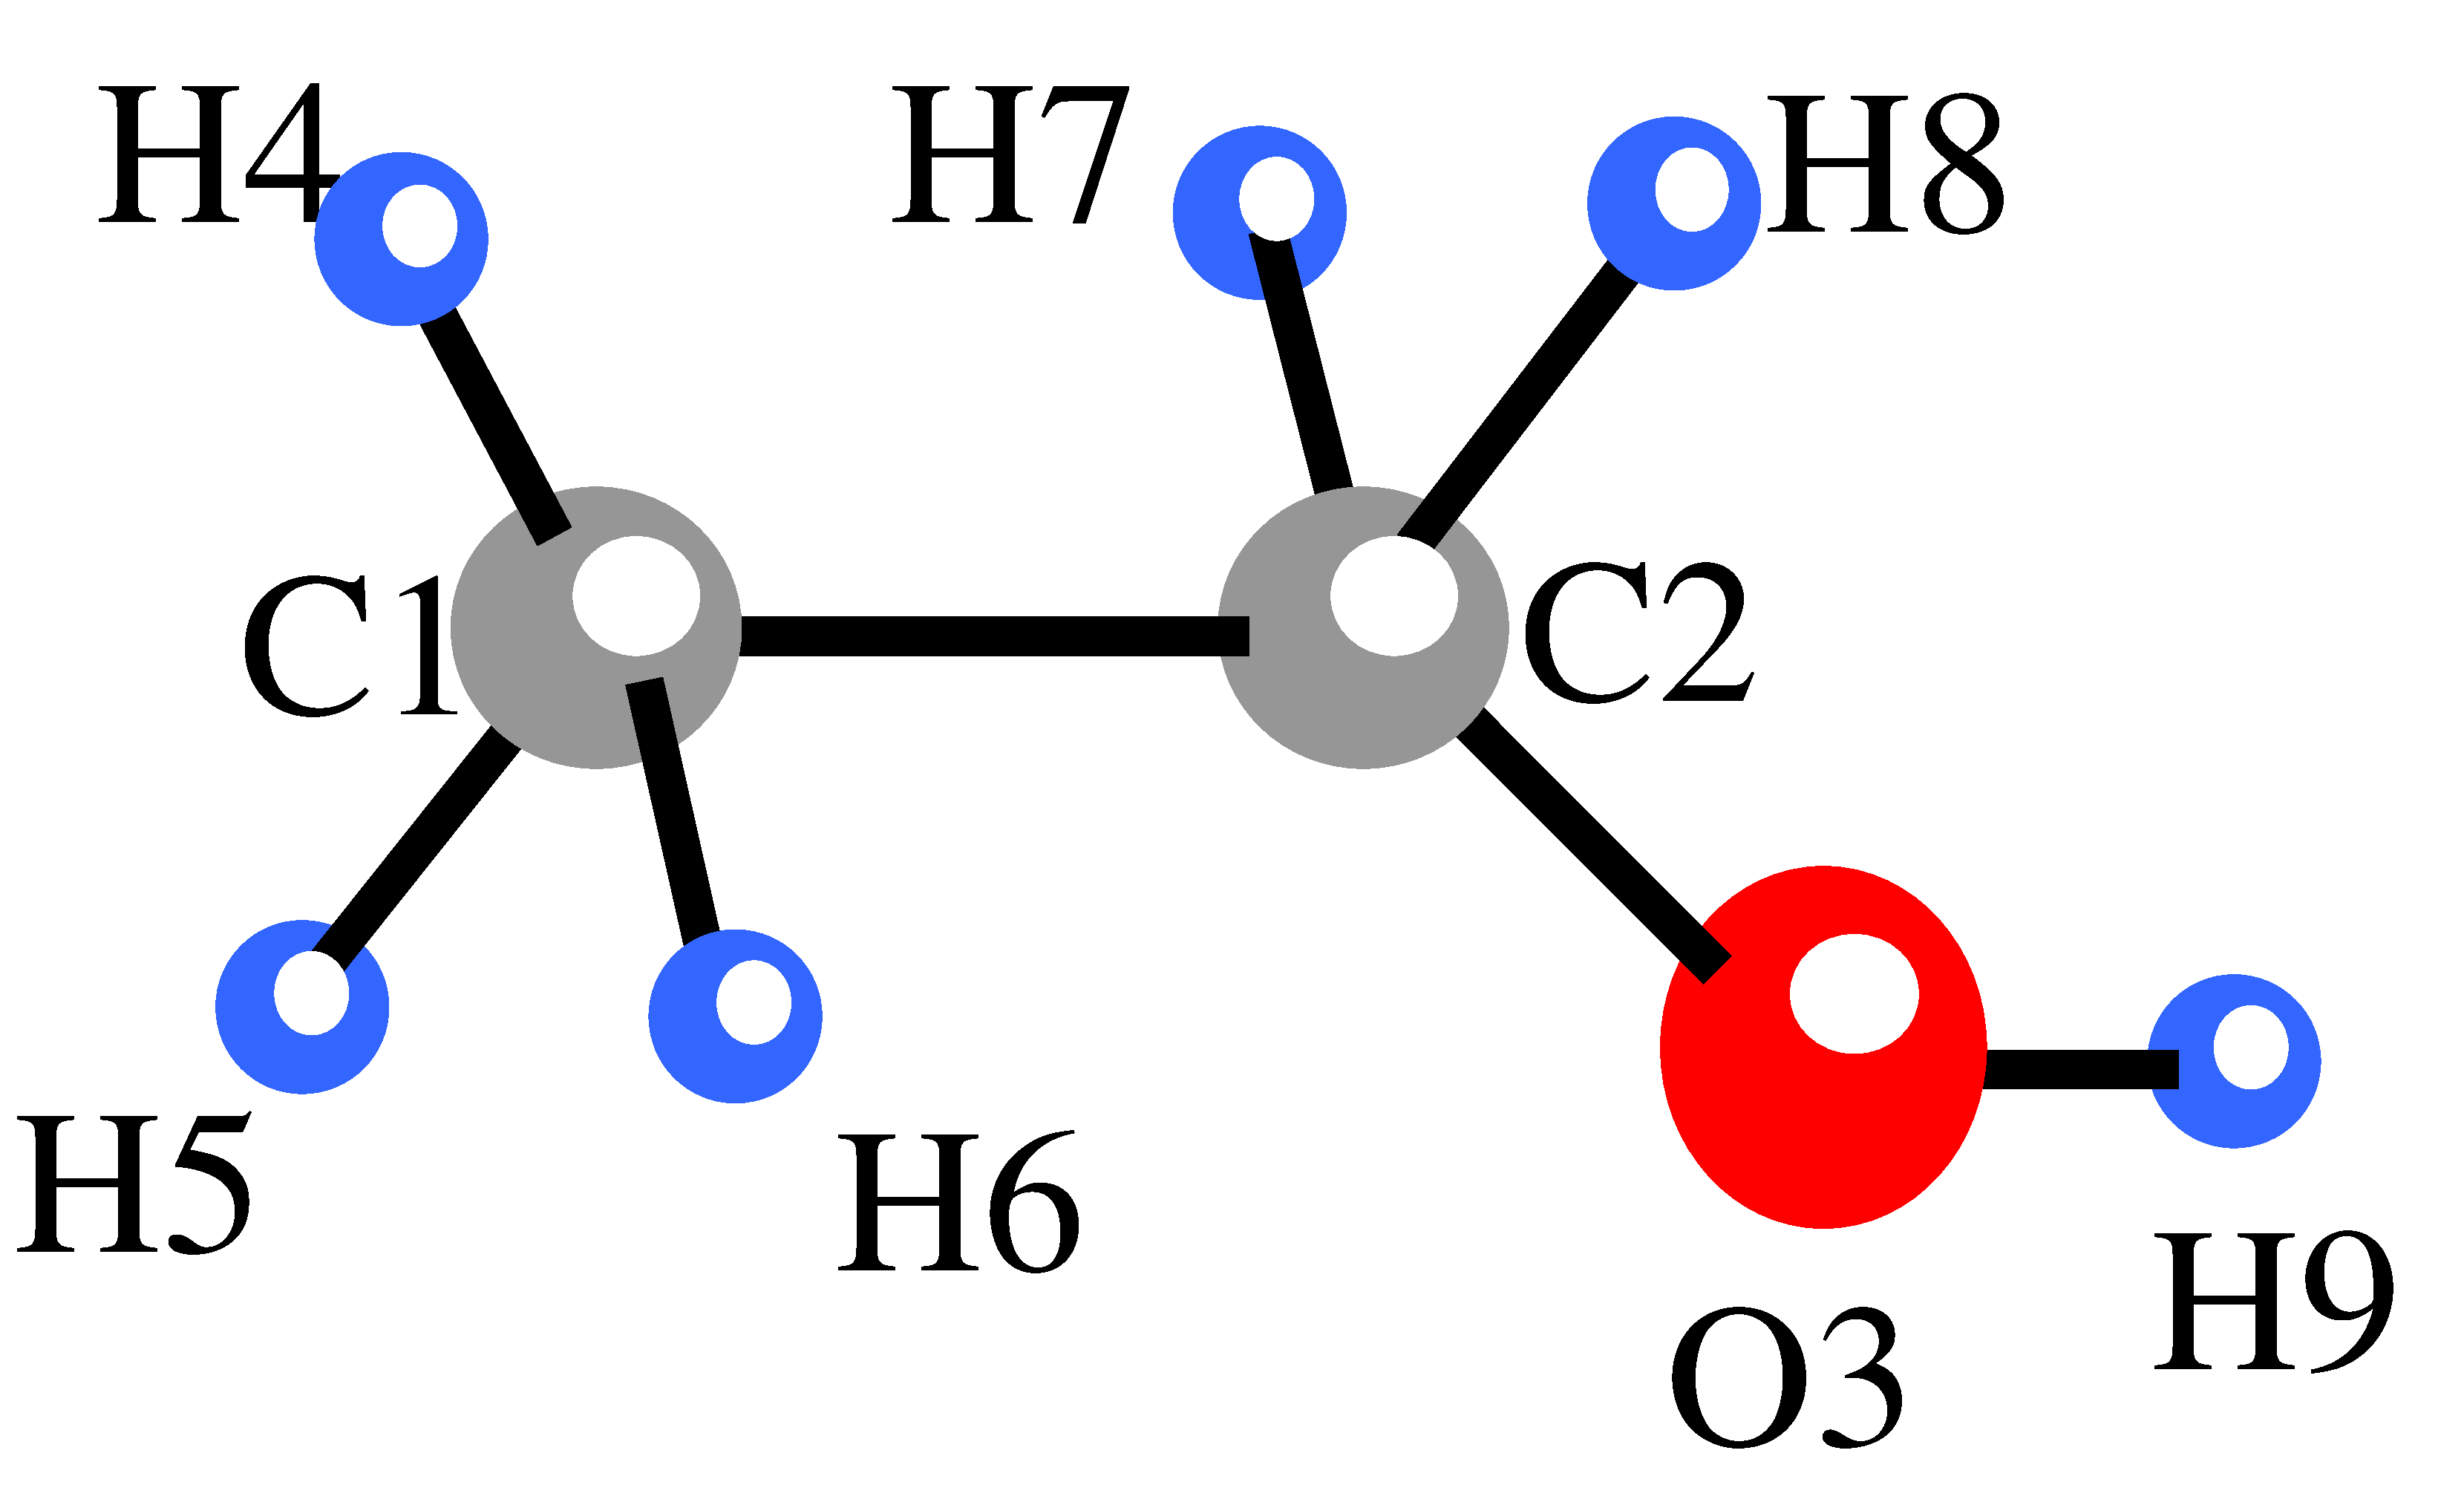
\includegraphics[%
  width=7cm,
  height=4.5cm]{mm9.eps}\end{center}

\noindent \texttt{\textit{\&two\_body\_list }}

\texttt{\textit{1 2}}

\texttt{\textit{1 4 }}

\texttt{\textit{1 5 }}

\texttt{\textit{1 6 }}

\texttt{\textit{2 3}}

\texttt{\textit{2 7 }}

\texttt{\textit{2 8 }}

\texttt{\textit{3 9 }}~\\
\texttt{\textit{/two\_body\_list }}~\\
\texttt{\textit{\&three\_body\_list }}

\texttt{\textit{2 1 4 }}

\texttt{\textit{2 1 5 }}

\texttt{\textit{2 1 6 }}

\texttt{\textit{4 1 5 }}

\texttt{\textit{4 1 6 }}

\texttt{\textit{5 1 6 }}

\texttt{\textit{1 2 3}}

\texttt{\textit{1 2 7 }}

\texttt{\textit{1 2 8 }}

\texttt{\textit{3 2 7 }}

\texttt{\textit{3 2 8 }}

\texttt{\textit{7 2 8}}

\texttt{\textit{2 3 9}}~\\
\texttt{\textit{/three\_body\_list}}~\\
\texttt{\textit{\&four\_body\_list }}

\texttt{\textit{4 1 2 3 }}

\texttt{\textit{4 1 2 7}}

\texttt{\textit{4 1 2 8}}

\texttt{\textit{5 1 2 3}}

\texttt{\textit{5 1 2 7}}

\texttt{\textit{5 1 2 8 }}

\texttt{\textit{6 1 2 3}}

\texttt{\textit{6 1 2 7 }}

\texttt{\textit{6 1 2 8 }}

\texttt{\textit{1 2 3 9}}

\texttt{\textit{7 2 3 9 }}

\texttt{\textit{8 2 3 9 }}~\\
\texttt{\textit{/four\_body\_list }}~\\
\texttt{\textit{\&bnd\_bnd\_list}}

\texttt{\textit{2 4 1 2 5 }}

\texttt{\textit{2 4 1 2 6}}

\texttt{\textit{2 4 1 4 5 }}

\texttt{\textit{2 4 1 4 6 }}

\texttt{\textit{2 4 1 5 6 }}

\texttt{\textit{2 5 1 2 6 }}

\texttt{\textit{2 5 1 4 5 }}

\texttt{\textit{2 5 1 4 6 }}

\texttt{\textit{2 5 1 5 6 }}

\texttt{\textit{2 6 1 4 5 }}

\texttt{\textit{2 6 1 4 6 }}

\texttt{\textit{2 6 1 5 6 }}

\texttt{\textit{4 5 1 4 6}}

\texttt{\textit{4 5 1 5 6 }}

\texttt{\textit{4 6 1 5 6 }}

\texttt{\textit{1 3 2 1 7}}

\texttt{\textit{1 3 2 1 8}}

\texttt{\textit{1 3 2 3 7}}

\texttt{\textit{1 3 2 3 8 }}

\texttt{\textit{1 3 2 7 8 }}

\texttt{\textit{1 7 2 1 8}}

\texttt{\textit{1 7 2 3 7 }}

\texttt{\textit{1 7 2 3 8}}

\texttt{\textit{1 7 2 7 8 }}

\texttt{\textit{1 8 2 3 7}}

\texttt{\textit{1 8 2 3 8}}

\texttt{\textit{1 8 2 7 8}}

\texttt{\textit{3 7 2 3 8}}

\texttt{\textit{3 7 2 7 8}}

\texttt{\textit{3 8 2 7 8}}~\\
\texttt{\textit{/bnd\_bnd\_list}}\texttt{}~\\
\texttt{\textit{\&str\_bnd\_list }}

\texttt{\textit{2 1 4 }}

\texttt{\textit{2 1 5 }}

\texttt{\textit{2 1 6}}

\texttt{\textit{4 1 5}}

\texttt{\textit{4 1 6 }}

\texttt{\textit{5 1 6}}

\texttt{\textit{1 2 3}}

\texttt{\textit{1 2 7}}

\texttt{\textit{1 2 8}}

\texttt{\textit{3 2 7}}

\texttt{\textit{3 2 8}}

\texttt{\textit{7 2 8}}

\texttt{\textit{2 3 9 }}~\\
\texttt{\textit{/str\_bnd\_list}} \texttt{}~\\
\texttt{\textit{\&str\_trs\_list}}

\texttt{\textit{4 1 2 3}}

\texttt{\textit{4 1 2 7}}

\texttt{\textit{4 1 2 8}}

\texttt{\textit{5 1 2 3}}

\texttt{\textit{5 1 2 7}}

\texttt{\textit{5 1 2 8}}

\texttt{\textit{6 1 2 3}}

\texttt{\textit{6 1 2 7}}

\texttt{\textit{6 1 2 8}}

\texttt{\textit{1 2 3 9}}

\texttt{\textit{7 2 3 9}}

\texttt{\textit{8 2 3 9}}~\\
\texttt{\textit{/str\_trs\_list }}

\textit{The examples of whole input files are presented in Appendixes
3 and 4}


\section{Execution of molecular mechanics task}

~~~~Because of Molecular Mechanics module is the part of ParaGauss
anyone who wants to run a molecular mechanics job has besides a molecular
mechanics input (\textbf{molmech.inp}) to have standard ParaGauss
input file (\textbf{input}). ParaGauss input can contain only two
namelists - \textbf{OPERATIONS} and \textbf{PVMOPTIONS} or \textbf{TASKS}
and \textbf{PVMOPTIONS}. 

\textit{Below the examples of ParaGauss input file are : }\\
\texttt{\textit{\&operations }}

\texttt{\textit{operations\_mol\_mech = true }}~\\
\texttt{\textit{/operations }}~\\
\texttt{\textit{\&pvmoptions}}

\texttt{\textit{n\_procs = 1 }}~\\
\texttt{\textit{/pvmoptions}}\textit{}\\
\textit{or }\\
\texttt{\textit{\&tasks }}

\texttt{\textit{task = {}``Mol\_mech'' }}~\\
\texttt{\textit{/tasks }}~\\
\texttt{\textit{\&pvmoptions}}

\texttt{\textit{n\_procs = 1 }}~\\
\texttt{\textit{/pvmoptions }}


\section{QM/MM calculation with the molecular mechanics module.}

~~~~Currently three different hybrid methods combining QM and
MM aproaches (QM/MM) can be done with \noun{ParaGauss}. One of them
is the famous the EPE (covEPE) method which can be activated if the
parameter \textbf{OPERATIONS\_QM\_EPE} is equal \textbf{TRUE}. The
EPE method uses its own molecular mechanics module oriented at calculations
of defects in solids. A description of the EPE method can be found
in original papers and a user manual (?). Two other QM/MM methods
are the variant of Morocuma IMOMM method and the additive scheme (just
QM/MM in a text below) suitable for calculations of processes in a
solvent. The last approach can also be used covalent systems expoloited
{}``pseudobond'' approaches.

A description of the the IMOMM method currently implemented into \noun{ParaGauss}
is not the subject of this document. It can be found elsewhere (see,
for example, the thesis of Andr� Woiterski or QM/MM (DL\_POLY\_2)
User Guide). Just remember, with the molecular mechanics module any
interface scripts and programs are no longer used. A whole a IMOMM
task is managed now by \noun{ParaGauss}. It makes a IMOMM job simpler
for users and more stabile. Optimization of geometry by IMOMM method
now looks like a standard optimization run. 

To start the IMOMM job anyone has to have four input files:

\begin{enumerate}
\item {}``\textbf{master.input}'' file,
\item standard \noun{ParaGauss} \textbf{input} file and
\item two input files for molecular mechanics module - {}``\textbf{molmech.inp.2}''
and {}``\textbf{molmech.inp.3}''.
\end{enumerate}
~~~~~{}``\textbf{Master.input}'' file describes the entire
QM/MM system and its dividing in quantum mechanical and molecular
mechanical parts. It is based on a standard \textbf{GX} file and usually
contains initial coordinates of the system. Therefore to start the
IMOMM task it is not necessary to have \textbf{GX} file but to continue
the task the GX file has to be in the input directory. 

{}``\textbf{Input}'' is used to handle a IMOMM job and calculate
quantum mechanically the central part of a IMOMM system. The IMOMM
task will start if in the namelist \textbf{OPERATIONS} the parameter
\textbf{OPERATIONS\_QM\_MM\_NEW} is equal \textbf{TRUE} and of course
\textbf{OPERATIONS\_GEO\_OPT} also is specified as \textbf{TRUE}.
If one prefers to use the namelist \textbf{TASKS} then in combination
with parameter \textbf{TASK=''GeoOpt''} parameter \textbf{QM\_MM\_NEW=TRUE}
has to be defined. 

The files {}``\textbf{molmech.inp.2}'' and {}``\textbf{molmech.inp.3}''
define the central and the entire parts of QM/MM system for molecular
mechanics calculations. 

The QM/MM approach (or explicit solvent model) is the newest variant
of hybrid methods within \noun{ParaGauss} and we will spend more
time to describe how to run it. A QM/MM task looks a bit simpler than
a IMOMM one. Three input files are needed to run a QM/MM task:

\begin{enumerate}
\item standard \noun{ParaGauss} \textbf{input} file,
\item input files for molecular mechanics module - {}``\textbf{molmech.inp''},
\item standard \textbf{GX} file.
\end{enumerate}
~~~~~\textbf{''Input''} as usual serves to describe the QM
part of the whole QM/MM system and manage the QM/MM task. As a IMOMM
job the QM/MM task is activated if either the parameter \textbf{OPERATIONS\_QM\_MM\_NEW}
(within \textbf{}the namelist \textbf{OPERATIONS}) or the parameter
\textbf{QM\_MM\_NEW} (within the namelist \textbf{TASKS}) is equal
\textbf{TRUE}. To choose between IMOMM and QM/MM tasks the new nemelist
\textbf{QMMM} has to be included within \textbf{{}``input''} file.
The namelist has only one parameter \textbf{METHOD}:\\
\texttt{\textbf{\&qmmm}}

\texttt{\textbf{method = {}``imomm'' or {}``qm+mm''}}~\\
\texttt{\textbf{/qmmm}}\\
\textbf{{}``Imomm''} is the default value. To choose the QM/MM task
\textbf{{}``qm+mm''} value has to be specified.

\textbf{{}``Molmech.\.{\i}np''} file contains the whole QM/MM system
and defines interactions within the MM subsystem and the MM and QM
atoms. Also it is possible to define MM interactions between QM atoms.
The names of QM and MM atoms has to be different.

\noun{Anyone has to remember QM atoms in} \textbf{\noun{{}``molmech.inp''}}
\noun{(and} \textbf{\noun{GX}} \noun{file also) has to be defined
in the beginning of a coordinates block. This convention help progrem
very easy to distinguish the QM and MM subsystems.}

The namelists \textbf{TASKS}, \textbf{OPT\_OPTIONS} and \textbf{HESS\_OPTIONS}
are not important for a QM/MM tasks and ignored.

The QM/MM approach can be combined with a continuum solvation model
(\textbf{COSMO}). But in a QM run the MM atoms are seen as point charges.
That is why no predefined van der Waals radii for them. To be able
to use \textbf{COSMO} model with the QM/MM task MM atoms has to be
named correctly (i.e. as atoms are named in Periodic table) otherwise
the QM/MM task is started without solvation model. 

The initial aim of the QM/MM aproach is to study processes in water.
To describe water solvent the \textbf{TIP3P} model is used. See Appendix
5 for details how define TIP3P model by \textbf{{}``molmech.inp''}
and \textbf{GX} files.


\section*{Appendix 1. Predefined atom names and covalent radii. }

\texttt{\textbf{Element ~~~~~Name ~~Covalent radius (�)}} \texttt{}~\\
\texttt{Hydrogen ~~~~~H\_~~~~~~~~~ 0.37 }~\\
\texttt{Helium ~~~~~~~HE~~~~~~~~~ 1.60}~\\
\texttt{Lithium ~~~~~~LI~~~~~~~~~ 0.68 }~\\
\texttt{Beryllium ~~~~BE~~~~~~~~~ 0.35 }~\\
\texttt{Boron ~~~~~~~~B\_~~~~~~~~~ 0.83 }~\\
\texttt{Carbon ~~~~~~~C\_~~~~~~~~~ 0.77}~\\
\texttt{Nitrogen ~~~~~N\_~~~~~~~~~ 0.75}~\\
\texttt{Oxygen ~~~~~~~O\_~~~~~~~~~ 0.73}~\\
\texttt{Fluorine ~~~~~F\_~~~~~~~~~ 0.71 }~\\
\texttt{Neon ~~~~~~~~~NE~~~~~~~~~ 1.12 }~\\
\texttt{Sodium ~~~~~~~NA~~~~~~~~~ 0.97}~\\
\texttt{Magnesium ~~~~MG~~~~~~~~~ 1.10}~\\
\texttt{Aluminum ~~~~~AL~~~~~~~~~ 1.35}~\\
\texttt{Silicon ~~~~~~SI~~~~~~~~~ 1.20 }~\\
\texttt{Phosphorus ~~~P\_~~~~~~~~~ 1.05 }~\\
\texttt{Sulfur ~~~~~~~S\_~~~~~~~~~ 1.02}~\\
\texttt{Chlorine ~~~~~CL~~~~~~~~~ 0.99 }~\\
\texttt{Argon ~~~~~~~~AR~~~~~~~~~ 1.54}~\\
\texttt{Potassium ~~~~K\_~~~~~~~~~ 1.33 }~\\
\texttt{Calcium ~~~~~~CA~~~~~~~~~ 0.99 }~\\
\texttt{Scandium ~~~~~SC~~~~~~~~~ 1.94}~\\
\texttt{Titanium ~~~~~TI~~~~~~~~~ 1.47}~\\
\texttt{Vanadium ~~~~~V\_~~~~~~~~~ 1.33}~\\
\texttt{Chromium ~~~~~CR~~~~~~~~~ 1.35 }~\\
\texttt{Manganese ~~~~MG~~~~~~~~~ 1.35}~\\
\texttt{Iron ~~~~~~~~~FE~~~~~~~~~ 1.34}~\\
\texttt{Cobalt ~~~~~~~CO~~~~~~~~~ 1.33}~\\
\texttt{Nickel ~~~~~~~NI~~~~~~~~~ 1.50}~\\
\texttt{Copper ~~~~~~~CU~~~~~~~~~ 1.52}~\\
\texttt{Zinc ~~~~~~~~~ZN~~~~~~~~~ 1.45}~\\
\texttt{Gallium ~~~~~~GA~~~~~~~~~ 1.22 }~\\
\texttt{Germanium ~~~~GE~~~~~~~~~ 1.17}~\\
\texttt{Arsenic ~~~~~~AS~~~~~~~~~ 1.21}~\\
\texttt{Selenium ~~~~~SE~~~~~~~~~ 1.22}~\\
\texttt{Bromine ~~~~~~BR~~~~~~~~~ 1.21}~\\
\texttt{Krypton ~~~~~~KR~~~~~~~~~ 1.89}~\\
\texttt{Rubidium ~~~~~RB~~~~~~~~~ 1.47}~\\
\texttt{Strontium ~~~~SR~~~~~~~~~ 1.12}~\\
\texttt{Yttrium ~~~~~~Y\_~~~~~~~~~ 1.78 }~\\
\texttt{Zirconium ~~~~ZR~~~~~~~~~ 1.56}~\\
\texttt{Niobium ~~~~~~NB~~~~~~~~~ 1.48}~\\
\texttt{Molybdenum ~~~MO~~~~~~~~~ 1.47}~\\
\texttt{Technetium ~~~TC~~~~~~~~~ 1.35}~\\
\texttt{Ruthenium ~~~~RU~~~~~~~~~ 1.40}~\\
\texttt{Rhodium ~~~~~~RH~~~~~~~~~ 1.45}~\\
\texttt{Palladium ~~~~PD~~~~~~~~~ 1.54}~\\
\texttt{Silver ~~~~~~~AG~~~~~~~~~ 1.59}~\\
\texttt{Cadmium ~~~~~~CD~~~~~~~~~ 1.69}~\\
\texttt{Indium ~~~~~~~IN~~~~~~~~~ 1.63}~\\
\texttt{Tin ~~~~~~~~~~SN~~~~~~~~~ 1.46 }~\\
\texttt{Antinomy ~~~~~SB~~~~~~~~~ 1.46}~\\
\texttt{Tellurium ~~~~TE~~~~~~~~~ 1.47}~\\
\texttt{Iodine ~~~~~~~I\_~~~~~~~~~ 1.40 }~\\
\texttt{Xenon ~~~~~~~~XE~~~~~~~~~ 1.33}~\\
\texttt{Cesium ~~~~~~~CS~~~~~~~~~ 1.67}~\\
\texttt{Barium ~~~~~~~BA~~~~~~~~~ 1.34}~\\
\texttt{Lanthanum ~~~~LA~~~~~~~~~ 1.87}~\\
\texttt{Cerium ~~~~~~~CE~~~~~~~~~ 1.83}~\\
\texttt{Praseodymium ~PR~~~~~~~~~ 1.82}~\\
\texttt{Neodymium ~~~~ND~~~~~~~~~ 1.81}~\\
\texttt{Promethium ~~~PM~~~~~~~~~ 1.80}~\\
\texttt{Samarium ~~~~~SM~~~~~~~~~ 1.80}~\\
\texttt{Europium ~~~~~EU~~~~~~~~~ 1.99 }~\\
\texttt{Gadolinium ~~~GD~~~~~~~~~ 1.79}~\\
\texttt{Terbium ~~~~~~TB~~~~~~~~~ 1.76 }~\\
\texttt{Dysprosium ~~~DY~~~~~~~~~ 1.75}~\\
\texttt{Holmium ~~~~~~HO~~~~~~~~~ 1.74}~\\
\texttt{Erbium ~~~~~~~ER~~~~~~~~~ 1.73}~\\
\texttt{Thulium ~~~~~~TM~~~~~~~~~ 1.72}~\\
\texttt{Ytterbium ~~~~YB~~~~~~~~~ 1.94}~\\
\texttt{Lutetium ~~~~~LU~~~~~~~~~ 1.72 }~\\
\texttt{Hafnium ~~~~~~HF~~~~~~~~~ 1.57}~\\
\texttt{Tantalum ~~~~~TA~~~~~~~~~ 1.43}~\\
\texttt{Tungsten ~~~~~W\_~~~~~~~~~ 1.37}~\\
\texttt{Rhenium ~~~~~~RE~~~~~~~~~ 1.35}~\\
\texttt{Osmium ~~~~~~~OS~~~~~~~~~ 1.37}~\\
\texttt{Iridium ~~~~~~IR~~~~~~~~~ 1.32}~\\
\texttt{Platinum ~~~~~PT~~~~~~~~~ 1.50}~\\
\texttt{Gold ~~~~~~~~~AU~~~~~~~~~ 1.50}~\\
\texttt{Mercury ~~~~~~HG~~~~~~~~~ 1.70}~\\
\texttt{Thallium ~~~~~TL~~~~~~~~~ 1.55}~\\
\texttt{Lead ~~~~~~~~~PB~~~~~~~~~ 1.54}~\\
\texttt{Bismuth ~~~~~~BI~~~~~~~~~ 1.54}~\\
\texttt{Polonium ~~~~~PO~~~~~~~~~ 1.68}~\\
\texttt{Astatine ~~~~~AT~~~~~~~~~ 1.45}~\\
\texttt{Radon ~~~~~~~~RN~~~~~~~~~ 1.90}~\\
\texttt{Francium ~~~~~FR~~~~~~~~~ 0.00}~\\
\texttt{Radium ~~~~~~~RA~~~~~~~~~ 1.90}~\\
\texttt{Actinium ~~~~~AC~~~~~~~~~ 1.88}~\\
\texttt{Thorium ~~~~~~TH~~~~~~~~~ 1.79}~\\
\texttt{Protactinium ~PA~~~~~~~~~ 1.61}~\\
\texttt{Uranium ~~~~~~U\_~~~~~~~~~ 1.58}~\\
\texttt{Neptunium ~~~~NP~~~~~~~~~ 1.55}~\\
\texttt{Plutonium ~~~~PU~~~~~~~~~ 1.53}~\\
\texttt{Americium ~~~~AM~~~~~~~~~ 1.51}~\\
\texttt{Curium ~~~~~~~CM~~~~~~~~~ 0.00}~\\
\texttt{Berkelium~~~~ BK~~~~~~~~~ 0.00}~\\
\texttt{Californium ~~CF~~~~~~~~~ 0.00}


\section*{Appendix 2. File format of user defined tabulated van der Waals potential. }

~~~~~The file containing user defined potential consists of \textbf{IDENT\_DATA}
namelist and the data describing potential in tabulated form. Also
any number of first lines can contain (if desirable) any useful information
that is actually ignored during reading in file data. Namelist \textbf{IDENT\_DATA}
consists of some parameters describing the type of tabulated potential.
At the moment for users only two of them are imporant. \textbf{}\\
\texttt{\textbf{\&ident\_data }}

\texttt{\textbf{n\_points = ??? }}

\texttt{\textbf{step ~~~~= ??? }}~\\
\texttt{\textbf{/ident\_data}}\\
\textbf{n\_points} - defines total number of points. It is recommended
to use the number of points per angstrom on the order of 50 to 100
for accurate representation of potential curve. \textbf{}\\
\textbf{Step} - defines distance (�) between nearest points. 

Potential data have to follow just after namelist \textbf{IDENT\_DATA}
(no any number of additional lines allowed). The potential data are
represented as a table consisting of five unformatted columns. The
first columns is the inter-atomic distance $r_{i}$. The two next
columns are \textbf{\textit{$g_{i}$}} and \textbf{\textit{$g_{i}^{\prime\prime}$}}
values of the repulsion part of van der Waals interaction. The last
two columns present \textbf{\textit{$h_{i}$}} and \textbf{\textit{$h_{i}^{\prime\prime}$}}
values of the attractive term (see paragraph 1.2.1). To avoid possible
problem \textbf{\textit{$r_{i}$}} should run from \textbf{$0$} to
\textbf{$rcut+0.5$} �. Of course if a potential function contains
a singularity at \textbf{$r_{i}=0$} a user can start the table with
the distance about 0.05-0.1 \textbf{}� because it is usual that atoms
are not closer each other than 0.5 \textbf{}�. 

\textit{Example:} \\
\texttt{\textit{-{}-{}-{}-{}-{}-{}-{}-{}-{}-{}-{}-{}-{}-{}-{}-{}-{}-{}-{}-{}-{}-{}-{}-{}-{}-{}-{}-{}-{}-{}-{}-{}-{}-{}-{}-{}-{}-{}-{}-{}-{}-{}-{}-{}-{}-{}-{}-{}-{}-{}-{}-{}-{}-{}-{}-
}}~\\
\texttt{\textit{This is only for example. }}~\\
\texttt{\textit{All data are not useable }}~\\
\texttt{\textit{\&ident\_data }}

\texttt{\textit{n\_points = 10 }}

\texttt{\textit{step = 1.0 }}~\\
\texttt{\textit{/ident\_data}}~\\
\texttt{\textit{0.0 1.0 2.0 1.0 2.0 }}~\\
\texttt{\textit{1.0 1.0 2.0 1.0 2.0 }}~\\
\texttt{\textit{2.0 1.0 2.0 1.0 2.0 }}~\\
\texttt{\textit{3.0 1.0 2.0 1.0 2.0}}~\\
\texttt{\textit{4.0 1.0 2.0 1.0 2.0 }}~\\
\texttt{\textit{5.0 1.0 2.0 1.0 2.0 }}~\\
\texttt{\textit{6.0 1.0 2.0 1.0 2.0}}~\\
\texttt{\textit{7.0 1.0 2.0 1.0 2.0 }}~\\
\texttt{\textit{8.0 1.0 2.0 1.0 2.0}}~\\
\texttt{\textit{9.0 1.0 2.0 1.0 2.0 }}~\\
\texttt{\textit{-{}-{}-{}-{}-{}-{}-{}-{}-{}-{}-{}-{}-{}-{}-{}-{}-{}-{}-{}-{}-{}-{}-{}-{}-{}-{}-{}-{}-{}-{}-{}-{}-{}-{}-{}-{}-{}-{}-{}-{}-{}-{}-{}-{}-{}-{}-{}-{}-{}-{}-{}-{}-{}-{}-{}-{}-{}-{}- }}


\section*{Appendix 3. Input file for ethanol simulation}

\texttt{\scriptsize \&tasks }{\scriptsize \par}

\texttt{\scriptsize \# job\_tasks=\char`\"{}energy\char`\"{} }{\scriptsize \par}

\texttt{\scriptsize \#job\_tasks=\char`\"{}gradients\char`\"{} }{\scriptsize \par}

\texttt{\scriptsize job\_tasks=\char`\"{}optimization to\_xyz\char`\"{}}~\\
\texttt{\scriptsize /tasks}~\\
\texttt{\scriptsize }~\\
\texttt{\scriptsize \&topic }{\scriptsize \par}

\texttt{\scriptsize job\_topic=\char`\"{}ethanol\char`\"{} }~\\
\texttt{\scriptsize /topic }~\\
\texttt{\scriptsize }~\\
\texttt{\scriptsize \&main\_options }{\scriptsize \par}

\texttt{\scriptsize rcut\_vdw=20.0 }{\scriptsize \par}

\texttt{\scriptsize coulomb=.false. }{\scriptsize \par}

\texttt{\scriptsize energy\_unit = \char`\"{}kcal/mol\char`\"{} }~\\
\texttt{\scriptsize /main\_options} \texttt{}~\\
\texttt{\scriptsize }~\\
\texttt{\scriptsize \&hess\_options }{\scriptsize \par}

\texttt{\scriptsize hess\_type=\char`\"{}analytical\char`\"{} }~\\
 \texttt{\scriptsize /hess\_options}~\\
\texttt{\scriptsize }~\\
\texttt{\scriptsize \&cartesian\_coor}~\\
\texttt{\scriptsize C -0.231579 -0.370841 -0.037475}~\\
\texttt{\scriptsize C 0.229441 0.373160 1.224850 }~\\
\texttt{\scriptsize O 0.868228 -0.551628 2.114423}~\\
\texttt{\scriptsize H0 0.619613 -0.833754 -0.565710 }~\\
\texttt{\scriptsize H0 -0.709445 0.352087 -0.754607 }~\\
\texttt{\scriptsize H0 -0.976393 -1.144198 0.191635}~\\
\texttt{\scriptsize H2 -0.628785 0.860022 1.736350 }~\\
\texttt{\scriptsize H2 0.952253 1.174538 0.962081}~\\
\texttt{\scriptsize H1 0.204846 -1.119563 2.483509 }~\\
\texttt{\scriptsize /cartesian\_coor }~\\
\texttt{}~\\
\texttt{\scriptsize \&species}{\scriptsize \par}

\texttt{\scriptsize name=\char`\"{}H0\char`\"{} }{\scriptsize \par}

\texttt{\scriptsize charge=0.0}{\scriptsize \par}

\texttt{\scriptsize vdw\_red\_fac=0.923}{\scriptsize \par}

\texttt{\scriptsize main\_name=\char`\"{}H\_\char`\"{}}~\\
\texttt{\scriptsize /species}~\\
\texttt{\scriptsize }~\\
\texttt{\scriptsize \&species}{\scriptsize \par}

\texttt{\scriptsize name=\char`\"{}H1\char`\"{} }{\scriptsize \par}

\texttt{\scriptsize charge=0.0 }{\scriptsize \par}

\texttt{\scriptsize vdw\_red\_fac=0.923}{\scriptsize \par}

\texttt{\scriptsize main\_name=\char`\"{}H\_\char`\"{} }~\\
\texttt{\scriptsize /species }~\\
\texttt{\scriptsize }~\\
\texttt{\scriptsize \&species}{\scriptsize \par}

\texttt{\scriptsize name=\char`\"{}H2\char`\"{}}{\scriptsize \par}

\texttt{\scriptsize charge=0.0}{\scriptsize \par}

\texttt{\scriptsize vdw\_red\_fac=0.923}{\scriptsize \par}

\texttt{\scriptsize main\_name=\char`\"{}H\_\char`\"{}}~\\
\texttt{\scriptsize /species}~\\
\texttt{\scriptsize }~\\
\texttt{\scriptsize \&species}{\scriptsize \par}

\texttt{\scriptsize name=\char`\"{}C\char`\"{} }{\scriptsize \par}

\texttt{\scriptsize charge=0.0}{\scriptsize \par}

\texttt{\scriptsize main\_name=\char`\"{}C\_\char`\"{}}~\\
\texttt{\scriptsize /species}~\\
\texttt{\scriptsize }~\\
\texttt{\scriptsize \&species}{\scriptsize \par}

\texttt{\scriptsize name=\char`\"{}O\char`\"{}}{\scriptsize \par}

\texttt{\scriptsize charge=0.0}{\scriptsize \par}

\texttt{\scriptsize main\_name=\char`\"{}O\_\char`\"{}}~\\
\texttt{\scriptsize /species }~\\
\texttt{\scriptsize }~\\
\texttt{\scriptsize \&potential}{\scriptsize \par}

\texttt{\scriptsize pot\_name=\char`\"{}quadr\_str\char`\"{} }{\scriptsize \par}

\texttt{\scriptsize atom\_name= \char`\"{}C\char`\"{}, \char`\"{}C\char`\"{}}{\scriptsize \par}

\texttt{\scriptsize ff\_parameter= 646.0212, -2471.03109, 4900.8783285,
1.5177 \#1.5247-0.007 c-c-o }~\\
\texttt{\scriptsize /potential }~\\
\texttt{\scriptsize }~\\
\texttt{\scriptsize \&potential}{\scriptsize \par}

\texttt{\scriptsize pot\_name=\char`\"{}quadr\_str\char`\"{}}{\scriptsize \par}

\texttt{\scriptsize atom\_name= \char`\"{}C\char`\"{}, \char`\"{}O\char`\"{} }{\scriptsize \par}

\texttt{\scriptsize ff\_parameter= 820.116 , -3136.94370, 6221.605005,
1.428 \#1.413+0.015 c-o-h }~\\
\texttt{\scriptsize /potential}~\\
\texttt{\scriptsize }~\\
\texttt{\scriptsize \&potential}{\scriptsize \par}

\texttt{\scriptsize pot\_name=\char`\"{}quadr\_str\char`\"{}}{\scriptsize \par}

\texttt{\scriptsize atom\_name= \char`\"{}H0\char`\"{}, \char`\"{}C\char`\"{}}{\scriptsize \par}

\texttt{\scriptsize ff\_parameter= 681.9912, -2608.61634, 5173.755741,
1.11088 \#1.112-(0.0028{*}0.4) h-c-c-o }~\\
\texttt{\scriptsize /potential }~\\
\texttt{\scriptsize }~\\
\texttt{\scriptsize \&potential }{\scriptsize \par}

\texttt{\scriptsize pot\_name=\char`\"{}quadr\_str\char`\"{}}{\scriptsize \par}

\texttt{\scriptsize atom\_name= \char`\"{}H2\char`\"{}, \char`\"{}C\char`\"{}}{\scriptsize \par}

\texttt{\scriptsize ff\_parameter= 681.9912, -2608.61634, 5173.755741,
1.1092 \#1.112-0.0028 h-c-o }~\\
\texttt{\scriptsize /potential}~\\
\texttt{\scriptsize }~\\
\texttt{\scriptsize \&potential }{\scriptsize \par}

\texttt{\scriptsize pot\_name=\char`\"{}quadr\_str\char`\"{}}{\scriptsize \par}

\texttt{\scriptsize atom\_name= \char`\"{}H1\char`\"{}, \char`\"{}O\char`\"{}}{\scriptsize \par}

\texttt{\scriptsize ff\_parameter= 1097.8044,-4199.10183, 8328.2186295,
0.947}~\\
\texttt{\scriptsize /potential }~\\
\texttt{\scriptsize }~\\
\texttt{\scriptsize \&two\_body\_list }{\scriptsize \par}

\texttt{\scriptsize 1 2}{\scriptsize \par}

\texttt{\scriptsize 1 4 }{\scriptsize \par}

\texttt{\scriptsize 1 5}{\scriptsize \par}

\texttt{\scriptsize 1 6}{\scriptsize \par}

\texttt{\scriptsize 2 3}{\scriptsize \par}

\texttt{\scriptsize 2 7}{\scriptsize \par}

\texttt{\scriptsize 2 8}{\scriptsize \par}

\texttt{\scriptsize 3 9}~\\
\texttt{\scriptsize /two\_body\_list}~\\
\texttt{\scriptsize }~\\
\texttt{\scriptsize \&potential}{\scriptsize \par}

\texttt{\scriptsize pot\_name=\char`\"{}six\_bnd\char`\"{}}{\scriptsize \par}

\texttt{\scriptsize atom\_name= \char`\"{}C\char`\"{},\char`\"{}C\char`\"{},
\char`\"{}H0\char`\"{} }{\scriptsize \par}

\texttt{\scriptsize ff\_parameter= 0.0258587324,-5.430333804e-4,2.8961780288e-6,-4.52527817e-8,1.7066763384e-9,110.7}~\\
\texttt{\scriptsize /potential }~\\
\texttt{\scriptsize }~\\
\texttt{\scriptsize \&potential }{\scriptsize \par}

\texttt{\scriptsize pot\_name=\char`\"{}six\_bnd\char`\"{} }{\scriptsize \par}

\texttt{\scriptsize atom\_name= \char`\"{}C\char`\"{},\char`\"{}C\char`\"{},
\char`\"{}H2\char`\"{} }{\scriptsize \par}

\texttt{\scriptsize ff\_parameter= 0.0258587324,-5.430333804e-4,2.8961780288e-6,-4.52527817e-8,1.7066763384e-9,109.31
}~\\
\texttt{\scriptsize /potential }~\\
\texttt{}~\\
\texttt{\scriptsize \&potential }{\scriptsize \par}

\texttt{\scriptsize pot\_name=\char`\"{}six\_bnd\char`\"{} }{\scriptsize \par}

\texttt{\scriptsize atom\_name= \char`\"{}C\char`\"{},\char`\"{}C\char`\"{},
\char`\"{}O\char`\"{} }{\scriptsize \par}

\texttt{\scriptsize ff\_parameter= 0.0363775388,-7.639283148e-4,4.0742843456e-6,-6.36606929e-8,2.4009175608e-9,107.9
}~\\
\texttt{\scriptsize /potential }~\\
\texttt{\scriptsize }~\\
\texttt{\scriptsize \&potential}{\scriptsize \par}

\texttt{\scriptsize pot\_name=\char`\"{}six\_bnd\char`\"{}}{\scriptsize \par}

\texttt{\scriptsize atom\_name= \char`\"{}H1\char`\"{},\char`\"{}O\char`\"{},
\char`\"{}C\char`\"{} }{\scriptsize \par}

\texttt{\scriptsize ff\_parameter= 0.0328712700,-6.902966700e-4,3.6815822400e-6,-5.75247225e-8,2.1695038200e-9,106.8
}~\\
\texttt{\scriptsize /potential }~\\
\texttt{\scriptsize }~\\
\texttt{\scriptsize \&potential}{\scriptsize \par}

\texttt{\scriptsize pot\_name=\char`\"{}six\_bnd\char`\"{}}{\scriptsize \par}

\texttt{\scriptsize atom\_name= \char`\"{}H0\char`\"{},\char`\"{}C\char`\"{},
\char`\"{}H0\char`\"{}}{\scriptsize \par}

\texttt{\scriptsize ff\_parameter= 0.0241055980,-5.062175580e-4,2.6998269760e-6,-4.21847965e-8,1.5909694680e-9,107.8
}~\\
\texttt{\scriptsize /potential}~\\
\texttt{\scriptsize }~\\
\texttt{\scriptsize \&potential}{\scriptsize \par}

\texttt{\scriptsize pot\_name=\char`\"{}six\_bnd\char`\"{} }{\scriptsize \par}

\texttt{\scriptsize atom\_name= \char`\"{}H2\char`\"{},\char`\"{}C\char`\"{},
\char`\"{}H2\char`\"{} }{\scriptsize \par}

\texttt{\scriptsize ff\_parameter= 0.0241055980,-5.062175580e-4,2.6998269760e-6,-4.21847965e-8,1.5909694680e-9,107.6}~\\
\texttt{\scriptsize /potential}~\\
\texttt{\scriptsize }~\\
\texttt{\scriptsize \&potential}{\scriptsize \par}

\texttt{\scriptsize pot\_name=\char`\"{}six\_bnd\char`\"{}}{\scriptsize \par}

\texttt{\scriptsize atom\_name= \char`\"{}H2\char`\"{},\char`\"{}C\char`\"{},
\char`\"{}O\char`\"{}}{\scriptsize \par}

\texttt{\scriptsize ff\_parameter= 0.0359392552,-7.547243592e-4,4.0251965824e-6,-6.28936966e-8,2.3719908432e-9,108.9
}~\\
\texttt{\scriptsize /potential }~\\
\texttt{\scriptsize }~\\
\texttt{\scriptsize \&three\_body\_list}{\scriptsize \par}

\texttt{\scriptsize 2 1 4}{\scriptsize \par}

\texttt{\scriptsize 2 1 5}{\scriptsize \par}

\texttt{\scriptsize 2 1 6}{\scriptsize \par}

\texttt{\scriptsize 4 1 5}{\scriptsize \par}

\texttt{\scriptsize 4 1 6}{\scriptsize \par}

\texttt{\scriptsize 5 1 6 }{\scriptsize \par}

\texttt{\scriptsize 1 2 3}{\scriptsize \par}

\texttt{\scriptsize 1 2 7}{\scriptsize \par}

\texttt{\scriptsize 1 2 8}{\scriptsize \par}

\texttt{\scriptsize 3 2 7}{\scriptsize \par}

\texttt{\scriptsize 3 2 8}{\scriptsize \par}

\texttt{\scriptsize 7 2 8}{\scriptsize \par}

\texttt{\scriptsize 2 3 9}~\\
\texttt{\scriptsize /three\_body\_list }~\\
\texttt{\scriptsize }~\\
\texttt{\scriptsize \&potential}{\scriptsize \par}

\texttt{\scriptsize pot\_name=\char`\"{}tripl\_cos\char`\"{}}{\scriptsize \par}

\texttt{\scriptsize atom\_name= \char`\"{}H0\char`\"{},\char`\"{}C\char`\"{},\char`\"{}C\char`\"{},
\char`\"{}O\char`\"{}}{\scriptsize \par}

\texttt{\scriptsize ff\_parameter= 0.00, 0.00, 0.30}~\\
\texttt{\scriptsize /potential}~\\
\texttt{\scriptsize }~\\
\texttt{\scriptsize \&potential }{\scriptsize \par}

\texttt{\scriptsize pot\_name=\char`\"{}tripl\_cos\char`\"{} }{\scriptsize \par}

\texttt{\scriptsize atom\_name= \char`\"{}H0\char`\"{},\char`\"{}C\char`\"{},\char`\"{}C\char`\"{},
\char`\"{}H2\char`\"{} }{\scriptsize \par}

\texttt{\scriptsize ff\_parameter= 0.00,0.00,0.238 }~\\
\texttt{\scriptsize /potential }~\\
\texttt{\scriptsize }~\\
\texttt{\scriptsize \&potential}{\scriptsize \par}

\texttt{\scriptsize pot\_name=\char`\"{}tripl\_cos\char`\"{}}{\scriptsize \par}

\texttt{\scriptsize atom\_name= \char`\"{}C\char`\"{},\char`\"{}C\char`\"{},\char`\"{}O\char`\"{},
\char`\"{}H1\char`\"{}}{\scriptsize \par}

\texttt{\scriptsize ff\_parameter= 0.40, 0.00, 0.10}~\\
\texttt{\scriptsize /potential}~\\
\texttt{\scriptsize }~\\
\texttt{\scriptsize \&potential}{\scriptsize \par}

\texttt{\scriptsize pot\_name=\char`\"{}tripl\_cos\char`\"{} }{\scriptsize \par}

\texttt{\scriptsize atom\_name= \char`\"{}H1\char`\"{},\char`\"{}O\char`\"{},\char`\"{}C\char`\"{},
\char`\"{}H2\char`\"{}}{\scriptsize \par}

\texttt{\scriptsize ff\_parameter= 0.00,0.00,0.20}~\\
\texttt{\scriptsize /potential}~\\
\texttt{\scriptsize }~\\
\texttt{\scriptsize \&four\_body\_list}{\scriptsize \par}

\texttt{\scriptsize 4 1 2 3}{\scriptsize \par}

\texttt{\scriptsize 4 1 2 7}{\scriptsize \par}

\texttt{\scriptsize 4 1 2 8 }{\scriptsize \par}

\texttt{\scriptsize 5 1 2 3}{\scriptsize \par}

\texttt{\scriptsize 5 1 2 7}{\scriptsize \par}

\texttt{\scriptsize 5 1 2 8}{\scriptsize \par}

\texttt{\scriptsize 6 1 2 3}{\scriptsize \par}

\texttt{\scriptsize 6 1 2 7}{\scriptsize \par}

\texttt{\scriptsize 6 1 2 8}{\scriptsize \par}

\texttt{\scriptsize 1 2 3 9}{\scriptsize \par}

\texttt{\scriptsize 7 2 3 9}{\scriptsize \par}

\texttt{\scriptsize 8 2 3 9}~\\
\texttt{\scriptsize /four\_body\_list }~\\
\texttt{\scriptsize }~\\
\texttt{\scriptsize \&potential}{\scriptsize \par}

\texttt{\scriptsize pot\_name=\char`\"{}bnd\_bnd\char`\"{}}{\scriptsize \par}

\texttt{\scriptsize atom\_name= \char`\"{}C\char`\"{},\char`\"{}H0\char`\"{},\char`\"{}C\char`\"{},\char`\"{}C\char`\"{},\char`\"{}H0\char`\"{}}{\scriptsize \par}

\texttt{\scriptsize ff\_parameter= -0.0039445524, 110.7, 110.7}~\\
 \texttt{\scriptsize /potential}~\\
\texttt{\scriptsize }~\\
\texttt{\scriptsize \&potential }{\scriptsize \par}

\texttt{\scriptsize pot\_name=\char`\"{}bnd\_bnd\char`\"{}}{\scriptsize \par}

\texttt{\scriptsize atom\_name= \char`\"{}C\char`\"{},\char`\"{}H2\char`\"{},\char`\"{}C\char`\"{},\char`\"{}C\char`\"{},\char`\"{}H2\char`\"{}}{\scriptsize \par}

\texttt{\scriptsize ff\_parameter= -0.0039445524, 109.31, 109.31}~\\
\texttt{\scriptsize /potential}~\\
\texttt{\scriptsize }~\\
\texttt{\scriptsize \# \&potential }{\scriptsize \par}

\texttt{\scriptsize \# pot\_name=\char`\"{}bnd\_bnd\char`\"{} }{\scriptsize \par}

\texttt{\scriptsize \# atom\_name= \char`\"{}C\char`\"{},\char`\"{}H0\char`\"{},\char`\"{}C\char`\"{},\char`\"{}H0\char`\"{},\char`\"{}H0\char`\"{} }{\scriptsize \par}

\texttt{\scriptsize \# ff\_parameter= 0.0000, 110.7, 107.8 }~\\
\texttt{\scriptsize \# /potential }~\\
\texttt{\scriptsize }~\\
\texttt{\scriptsize \# \&potential}{\scriptsize \par}

\texttt{\scriptsize \# pot\_name=\char`\"{}bnd\_bnd\char`\"{} }{\scriptsize \par}

\texttt{\scriptsize \# atom\_name= \char`\"{}C\char`\"{},\char`\"{}H2\char`\"{},\char`\"{}C\char`\"{},\char`\"{}H2\char`\"{},\char`\"{}H2\char`\"{}}{\scriptsize \par}

\texttt{\scriptsize \# ff\_parameter= 0.0000, 109.31, 107.6 }~\\
\texttt{\scriptsize \# /potential}~\\
\texttt{\scriptsize }~\\
\texttt{\scriptsize \# \&potential}{\scriptsize \par}

\texttt{\scriptsize \# pot\_name=\char`\"{}bnd\_bnd\char`\"{}}{\scriptsize \par}

\texttt{\scriptsize \# atom\_name= \char`\"{}H0\char`\"{},\char`\"{}H0\char`\"{},\char`\"{}C\char`\"{},\char`\"{}H0\char`\"{},\char`\"{}H0\char`\"{}}{\scriptsize \par}

\texttt{\scriptsize \# ff\_parameter= 0.0000, 107.8, 107.8}~\\
\texttt{\scriptsize \# /potential }~\\
\texttt{\scriptsize }~\\
\texttt{\scriptsize \&potential}{\scriptsize \par}

\texttt{\scriptsize pot\_name=\char`\"{}bnd\_bnd\char`\"{} }{\scriptsize \par}

\texttt{\scriptsize atom\_name= \char`\"{}C\char`\"{},\char`\"{}O\char`\"{},\char`\"{}C\char`\"{},\char`\"{}C\char`\"{},\char`\"{}H2\char`\"{}}{\scriptsize \par}

\texttt{\scriptsize ff\_parameter= -0.00315564192, 107.9, 109.31}~\\
\texttt{\scriptsize /potential}~\\
\texttt{\scriptsize }~\\
\texttt{\scriptsize \# \&potential }{\scriptsize \par}

\texttt{\scriptsize \# pot\_name=\char`\"{}bnd\_bnd\char`\"{}}{\scriptsize \par}

\texttt{\scriptsize \# atom\_name= \char`\"{}C\char`\"{},\char`\"{}O\char`\"{},\char`\"{}C\char`\"{},\char`\"{}H2\char`\"{},\char`\"{}H2\char`\"{} }{\scriptsize \par}

\texttt{\scriptsize \# ff\_parameter= 0.00, 107.9, 107.6 }~\\
\texttt{\scriptsize \# /potential }~\\
\texttt{\scriptsize }~\\
\texttt{\scriptsize \&potential }{\scriptsize \par}

\texttt{\scriptsize pot\_name=\char`\"{}bnd\_bnd\char`\"{}}{\scriptsize \par}

\texttt{\scriptsize atom\_name= \char`\"{}C\char`\"{},\char`\"{}O\char`\"{},\char`\"{}C\char`\"{},\char`\"{}O\char`\"{},\char`\"{}H2\char`\"{}}{\scriptsize \par}

\texttt{\scriptsize ff\_parameter= -0.00315564192 , 107.9, 108.9}~\\
\texttt{\scriptsize /potential}~\\
\texttt{\scriptsize }~\\
\texttt{\scriptsize \&potential}{\scriptsize \par}

\texttt{\scriptsize pot\_name=\char`\"{}bnd\_bnd\char`\"{}}{\scriptsize \par}

\texttt{\scriptsize atom\_name= \char`\"{}C\char`\"{},\char`\"{}H2\char`\"{},\char`\"{}C\char`\"{},\char`\"{}O\char`\"{},\char`\"{}H2\char`\"{}}{\scriptsize \par}

\texttt{\scriptsize ff\_parameter= -0.0039445524 ,109.31, 108.9}~\\
\texttt{\scriptsize /potential}~\\
\texttt{\scriptsize }~\\
\texttt{\scriptsize \&potential}{\scriptsize \par}

\texttt{\scriptsize pot\_name=\char`\"{}bnd\_bnd\char`\"{}}{\scriptsize \par}

\texttt{\scriptsize atom\_name= \char`\"{}O\char`\"{},\char`\"{}H2\char`\"{},\char`\"{}C\char`\"{},\char`\"{}O\char`\"{},\char`\"{}H2\char`\"{}}{\scriptsize \par}

\texttt{\scriptsize ff\_parameter= -0.0039445524 ,108.9, 108.9}~\\
\texttt{\scriptsize /potential}~\\
\texttt{\scriptsize }~\\
\texttt{\scriptsize \# \&potential}{\scriptsize \par}

\texttt{\scriptsize \# pot\_name=\char`\"{}bnd\_bnd\char`\"{}}{\scriptsize \par}

\texttt{\scriptsize \# atom\_name= \char`\"{}O\char`\"{},\char`\"{}H2\char`\"{},\char`\"{}C\char`\"{},\char`\"{}H2\char`\"{},\char`\"{}H2\char`\"{}}{\scriptsize \par}

\texttt{\scriptsize \# ff\_parameter= 0.00,108.9, 107.6}~\\
\texttt{\scriptsize \# /potential}~\\
\texttt{\scriptsize }~\\
\texttt{\scriptsize \&bnd\_bnd\_list}{\scriptsize \par}

\texttt{\scriptsize 2 4 1 2 5}{\scriptsize \par}

\texttt{\scriptsize 2 4 1 2 6 }{\scriptsize \par}

\texttt{\scriptsize \# 2 4 1 4 5}{\scriptsize \par}

\texttt{\scriptsize \# 2 4 1 4 6}{\scriptsize \par}

\texttt{\scriptsize \# 2 4 1 5 6}{\scriptsize \par}

\texttt{\scriptsize 2 5 1 2 6 }{\scriptsize \par}

\texttt{\scriptsize \# 2 5 1 4 5}{\scriptsize \par}

\texttt{\scriptsize \# 2 5 1 4 6}{\scriptsize \par}

\texttt{\scriptsize \# 2 5 1 5 6}{\scriptsize \par}

\texttt{\scriptsize \# 2 6 1 4 5}{\scriptsize \par}

\texttt{\scriptsize \# 2 6 1 4 6}{\scriptsize \par}

\texttt{\scriptsize \# 2 6 1 5 6}{\scriptsize \par}

\texttt{\scriptsize \# 4 5 1 4 6}{\scriptsize \par}

\texttt{\scriptsize \# 4 5 1 5 6 }{\scriptsize \par}

\texttt{\scriptsize \# 4 6 1 5 6}{\scriptsize \par}

\texttt{\scriptsize 1 3 2 1 7}{\scriptsize \par}

\texttt{\scriptsize 1 3 2 1 8}{\scriptsize \par}

\texttt{\scriptsize 1 3 2 3 7}{\scriptsize \par}

\texttt{\scriptsize 1 3 2 3 8}{\scriptsize \par}

\texttt{\scriptsize \# 1 3 2 7 8}{\scriptsize \par}

\texttt{\scriptsize 1 7 2 1 8 }{\scriptsize \par}

\texttt{\scriptsize 1 7 2 3 7}{\scriptsize \par}

\texttt{\scriptsize 1 7 2 3 8}{\scriptsize \par}

\texttt{\scriptsize \# 1 7 2 7 8}{\scriptsize \par}

\texttt{\scriptsize 1 8 2 3 7}{\scriptsize \par}

\texttt{\scriptsize 1 8 2 3 8}{\scriptsize \par}

\texttt{\scriptsize \# 1 8 2 7 8}{\scriptsize \par}

\texttt{\scriptsize 3 7 2 3 8}{\scriptsize \par}

\texttt{\scriptsize \# 3 7 2 7 8}{\scriptsize \par}

\texttt{\scriptsize \# 3 8 2 7 8}~\\
\texttt{\scriptsize /bnd\_bnd\_list}~\\
\texttt{\scriptsize }~\\
\texttt{\scriptsize \&potential}{\scriptsize \par}

\texttt{\scriptsize pot\_name=\char`\"{}str\_bnd\char`\"{}}{\scriptsize \par}

\texttt{\scriptsize atom\_name= \char`\"{}H0\char`\"{},\char`\"{}C\char`\"{},\char`\"{}H0\char`\"{}}{\scriptsize \par}

\texttt{\scriptsize ff\_parameter= 0.000,1.11088,1.1108,107.8}~\\
\texttt{\scriptsize /potential}~\\
\texttt{\scriptsize }~\\
\texttt{\scriptsize \&potential}{\scriptsize \par}

\texttt{\scriptsize pot\_name=\char`\"{}str\_bnd\char`\"{}}{\scriptsize \par}

\texttt{\scriptsize atom\_name= \char`\"{}H2\char`\"{},\char`\"{}C\char`\"{},\char`\"{}H2\char`\"{}}{\scriptsize \par}

\texttt{\scriptsize ff\_parameter= 0.000,1.11088,1.1108,107.6}~\\
\texttt{\scriptsize /potential}~\\
\texttt{\scriptsize }~\\
\texttt{\scriptsize \&potential}{\scriptsize \par}

\texttt{\scriptsize pot\_name=\char`\"{}str\_bnd\char`\"{}}{\scriptsize \par}

\texttt{\scriptsize atom\_name= \char`\"{}H0\char`\"{},\char`\"{}C\char`\"{},\char`\"{}C\char`\"{}}{\scriptsize \par}

\texttt{\scriptsize ff\_parameter= 0.2008944,1.11088,1.5177, 110.7}~\\
\texttt{\scriptsize /potential}~\\
\texttt{\scriptsize }~\\
\texttt{\scriptsize \&potential}{\scriptsize \par}

\texttt{\scriptsize pot\_name=\char`\"{}str\_bnd\char`\"{}}{\scriptsize \par}

\texttt{\scriptsize atom\_name= \char`\"{}H2\char`\"{},\char`\"{}C\char`\"{},\char`\"{}C\char`\"{}}{\scriptsize \par}

\texttt{\scriptsize ff\_parameter= 0.2008944,1.1092, 1.5177, 109.31}~\\
\texttt{\scriptsize /potential}~\\
\texttt{\scriptsize }~\\
\texttt{\scriptsize \&potential}{\scriptsize \par}

\texttt{\scriptsize pot\_name=\char`\"{}str\_bnd\char`\"{}}{\scriptsize \par}

\texttt{\scriptsize atom\_name= \char`\"{}C\char`\"{},\char`\"{}C\char`\"{},\char`\"{}O\char`\"{}}{\scriptsize \par}

\texttt{\scriptsize ff\_parameter= 0.3264534, 1.5177, 1.428 , 107.9}~\\
\texttt{\scriptsize /potential}~\\
\texttt{\scriptsize }~\\
\texttt{\scriptsize \&potential}{\scriptsize \par}

\texttt{\scriptsize pot\_name=\char`\"{}str\_bnd\char`\"{}}{\scriptsize \par}

\texttt{\scriptsize atom\_name= \char`\"{}O\char`\"{},\char`\"{}C\char`\"{},\char`\"{}H2\char`\"{}}{\scriptsize \par}

\texttt{\scriptsize ff\_parameter= 0.2008944, 1.428,1.1092 , 108.9
}~\\
\texttt{\scriptsize /potential}~\\
\texttt{\scriptsize }~\\
\texttt{\scriptsize \&potential}{\scriptsize \par}

\texttt{\scriptsize pot\_name=\char`\"{}str\_bnd\char`\"{}}{\scriptsize \par}

\texttt{\scriptsize atom\_name= \char`\"{}C\char`\"{},\char`\"{}O\char`\"{},\char`\"{}H1\char`\"{}}{\scriptsize \par}

\texttt{\scriptsize ff\_parameter= 0.2260062, 1.428, 0.947, 106.8}~\\
\texttt{\scriptsize /potential}~\\
\texttt{\scriptsize }~\\
\texttt{\scriptsize \&str\_bnd\_list}{\scriptsize \par}

\texttt{\scriptsize 2 1 4}{\scriptsize \par}

\texttt{\scriptsize 2 1 5}{\scriptsize \par}

\texttt{\scriptsize 2 1 6}{\scriptsize \par}

\texttt{\scriptsize 4 1 5}{\scriptsize \par}

\texttt{\scriptsize 4 1 6}{\scriptsize \par}

\texttt{\scriptsize 5 1 6}{\scriptsize \par}

\texttt{\scriptsize 1 2 3}{\scriptsize \par}

\texttt{\scriptsize 1 2 7}{\scriptsize \par}

\texttt{\scriptsize 1 2 8}{\scriptsize \par}

\texttt{\scriptsize 3 2 7 }{\scriptsize \par}

\texttt{\scriptsize 3 2 8 }{\scriptsize \par}

\texttt{\scriptsize 7 2 8}{\scriptsize \par}

\texttt{\scriptsize 2 3 9}~\\
\texttt{\scriptsize /str\_bnd\_list}~\\
\texttt{\scriptsize }~\\
\texttt{\scriptsize \&potential}{\scriptsize \par}

\texttt{\scriptsize pot\_name=\char`\"{}str\_trs\char`\"{}}{\scriptsize \par}

\texttt{\scriptsize atom\_name= \char`\"{}H0\char`\"{},\char`\"{}C\char`\"{},\char`\"{}C\char`\"{},
\char`\"{}H2\char`\"{} }{\scriptsize \par}

\texttt{\scriptsize ff\_parameter= -0.707705, 1.5177 \#1.5247 }~\\
\texttt{\scriptsize /potential }~\\
\texttt{\scriptsize }~\\
\texttt{\scriptsize \&potential}{\scriptsize \par}

\texttt{\scriptsize pot\_name=\char`\"{}str\_trs\char`\"{}}{\scriptsize \par}

\texttt{\scriptsize atom\_name= \char`\"{}H0\char`\"{},\char`\"{}C\char`\"{},\char`\"{}C\char`\"{},
\char`\"{}O\char`\"{}}{\scriptsize \par}

\texttt{\scriptsize ff\_parameter= -0.707705, 1.5177 \#1.5247}~\\
\texttt{\scriptsize /potential}~\\
\texttt{\scriptsize }~\\
\texttt{\scriptsize \&potential}{\scriptsize \par}

\texttt{\scriptsize pot\_name=\char`\"{}str\_trs\char`\"{}}{\scriptsize \par}

\texttt{\scriptsize atom\_name= \char`\"{}C\char`\"{},\char`\"{}C\char`\"{},\char`\"{}O\char`\"{},
\char`\"{}H1\char`\"{}}{\scriptsize \par}

\texttt{\scriptsize ff\_parameter= -1.1995, 1.428 \#1.413}~\\
\texttt{\scriptsize /potential }~\\
\texttt{\scriptsize }~\\
\texttt{\scriptsize \&potential}{\scriptsize \par}

\texttt{\scriptsize pot\_name=\char`\"{}str\_trs\char`\"{}}{\scriptsize \par}

\texttt{\scriptsize atom\_name= \char`\"{}H2\char`\"{},\char`\"{}C\char`\"{},\char`\"{}O\char`\"{},
\char`\"{}H1\char`\"{}}{\scriptsize \par}

\texttt{\scriptsize ff\_parameter= -1.1995, 1.428 \#1.413}~\\
\texttt{\scriptsize /potential}~\\
\texttt{\scriptsize }~\\
\texttt{\scriptsize \&str\_trs\_list}{\scriptsize \par}

\texttt{\scriptsize 4 1 2 3}{\scriptsize \par}

\texttt{\scriptsize 4 1 2 7}{\scriptsize \par}

\texttt{\scriptsize 4 1 2 8}{\scriptsize \par}

\texttt{\scriptsize 5 1 2 3}{\scriptsize \par}

\texttt{\scriptsize 5 1 2 7}{\scriptsize \par}

\texttt{\scriptsize 5 1 2 8}{\scriptsize \par}

\texttt{\scriptsize 6 1 2 3}{\scriptsize \par}

\texttt{\scriptsize 6 1 2 7}{\scriptsize \par}

\texttt{\scriptsize 6 1 2 8}{\scriptsize \par}

\texttt{\scriptsize 1 2 3 9}{\scriptsize \par}

\texttt{\scriptsize 7 2 3 9}{\scriptsize \par}

\texttt{\scriptsize 8 2 3 9}~\\
\texttt{\scriptsize /str\_trs\_list}~\\
\texttt{\scriptsize }~\\
\texttt{\scriptsize \&potential}{\scriptsize \par}

\texttt{\scriptsize pot\_name=\char`\"{}buck\char`\"{}}{\scriptsize \par}

\texttt{\scriptsize atom\_name= \char`\"{}H0\char`\"{},\char`\"{}O\char`\"{}}{\scriptsize \par}

\texttt{\scriptsize ff\_parameter= 6320.6075657,0.286667, 128.0778938}~\\
\texttt{\scriptsize /potential }~\\
\texttt{\scriptsize }~\\
\texttt{\scriptsize \&potential}{\scriptsize \par}

\texttt{\scriptsize pot\_name=\char`\"{}buck\char`\"{} }{\scriptsize \par}

\texttt{\scriptsize atom\_name= \char`\"{}H0\char`\"{},\char`\"{}H2\char`\"{}}{\scriptsize \par}

\texttt{\scriptsize ff\_parameter= 3680.00, 0.27000, 52.057412}~\\
\texttt{\scriptsize /potential}~\\
\texttt{\scriptsize }~\\
\texttt{\scriptsize \&potential}{\scriptsize \par}

\texttt{\scriptsize pot\_name=\char`\"{}buck\char`\"{}}{\scriptsize \par}

\texttt{\scriptsize atom\_name= \char`\"{}H0\char`\"{},\char`\"{}H1\char`\"{}}{\scriptsize \par}

\texttt{\scriptsize ff\_parameter= 3291.4920629, 0.2683333, 44.8634572}~\\
\texttt{\scriptsize /potential }~\\
\texttt{\scriptsize }~\\
\texttt{\scriptsize \&potential}{\scriptsize \par}

\texttt{\scriptsize pot\_name=\char`\"{}buck\char`\"{}}{\scriptsize \par}

\texttt{\scriptsize atom\_name= \char`\"{}H2\char`\"{},\char`\"{}H1\char`\"{}}{\scriptsize \par}

\texttt{\scriptsize ff\_parameter= 3291.4920629, 0.2683333, 44.8634572}~\\
\texttt{\scriptsize /potential}~\\
\texttt{\scriptsize }~\\
\texttt{\scriptsize \&potential}{\scriptsize \par}

\texttt{\scriptsize pot\_name=\char`\"{}buck\char`\"{}}{\scriptsize \par}

\texttt{\scriptsize atom\_name= \char`\"{}H1\char`\"{},\char`\"{}C\char`\"{}}{\scriptsize \par}

\texttt{\scriptsize ff\_parameter= 3824.3681831, 0.3033333, 108.7759020}~\\
\texttt{\scriptsize /potential}~\\
\texttt{\scriptsize }~\\
\texttt{\scriptsize \&electrostatic}{\scriptsize \par}

\texttt{\scriptsize electro\_type=\char`\"{}dipole-dipole\char`\"{}}~\\
\texttt{\scriptsize /end}~\\
\texttt{\scriptsize }~\\
\texttt{\scriptsize \&bond\_dipole}{\scriptsize \par}

\texttt{\scriptsize atom\_name= \char`\"{}C\char`\"{}, \char`\"{}O\char`\"{}}{\scriptsize \par}

\texttt{\scriptsize dip\_mom= 1.17}~\\
\texttt{\scriptsize /bond\_dipole}~\\
\texttt{\scriptsize }~\\
\texttt{\scriptsize \&bond\_dipole}{\scriptsize \par}

\texttt{\scriptsize atom\_name= \char`\"{}O\char`\"{}, \char`\"{}H1\char`\"{}}{\scriptsize \par}

\texttt{\scriptsize dip\_mom= -1.67}~\\
\texttt{\scriptsize /bond\_dipole}{\scriptsize \par}


\section*{Appendix 4. Input file to optimize chabazite}

\texttt{\&tasks }

\texttt{job\_tasks=\char`\"{}gradients \char`\"{} }

\texttt{\# job\_tasks=\char`\"{}hessian\char`\"{} }

\texttt{job\_tasks=\char`\"{}optimization\char`\"{}}~\\
\texttt{/tasks}~\\
\texttt{}~\\
\texttt{\&topic }

\texttt{job\_topic=\char`\"{}chabasite, Sierka-Sauer DFT FF, core-shell,
cell varing\char`\"{}}~\\
\texttt{/topic}~\\
\texttt{}~\\
\texttt{\&main\_options}

\texttt{rcut\_vdw=10.0 }

\texttt{coulomb=t }

\texttt{calc\_strain=t }

\texttt{energy\_unit = \char`\"{}eV\char`\"{} }

\texttt{angle\_unit=\char`\"{}radian\char`\"{} }

\texttt{minimal\_image = false}~\\
\texttt{/main\_options}~\\
\texttt{}~\\
\texttt{\&nb\_lists\_options}

\texttt{automatic\_nb\_lists = true }

\texttt{exclude\_1\_3 = f}~\\
\texttt{/nb\_lists\_options}~\\
\texttt{}~\\
\texttt{\&opt\_options}

\texttt{n\_iterations = 50}~\\
\texttt{/opt\_options}~\\
\texttt{}~\\
\texttt{\&hess\_options }

\texttt{\# hess\_type=\char`\"{}unit\char`\"{}}

\texttt{hess\_type=\char`\"{}analytical\char`\"{}}~\\
\texttt{/end}~\\
\texttt{}~\\
\texttt{\&cell}

\texttt{a=9.421 }

\texttt{b=9.421}

\texttt{c=9.421}

\texttt{alpha=94.20}

\texttt{beta=94.20}

\texttt{gamma=94.20}~\\
\texttt{/cell }~\\
\texttt{}~\\
\texttt{\&fractional\_coor}~\\
\texttt{Si 0.1044 0.3338 0.8749 }~\\
\texttt{Si 0.8749 0.1044 0.3338}~\\
\texttt{Si 0.3338 0.8749 0.1044}~\\
\texttt{Si 0.1251 0.6662 0.8956}~\\
\texttt{Si 0.6662 0.8956 0.1251}~\\
\texttt{Si 0.8956 0.1251 0.6662}~\\
\texttt{Si 0.8956 0.6662 0.1251}~\\
\texttt{Si 0.1251 0.8956 0.6662 }~\\
\texttt{Si 0.6662 0.1251 0.8956}~\\
\texttt{Si 0.8749 0.3338 0.1044}~\\
\texttt{Si 0.3338 0.1044 0.8749}~\\
\texttt{Si 0.1044 0.8749 0.3338}~\\
\texttt{O 0.2638 0.7362 0 }~\\
\texttt{O 0 0.2638 0.7362}~\\
\texttt{O 0.7362 0 0.2638}~\\
\texttt{O 0.7362 0.2638 0 }~\\
\texttt{O 0 0.7362 0.2638 }~\\
\texttt{O 0.2638 0 0.7362}~\\
\texttt{O 0.1548 0.8452 0.5}~\\
\texttt{O 0.5 0.1548 0.8452}~\\
\texttt{O 0.8452 0.5 0.1548}~\\
\texttt{O 0.8452 0.1548 0.5}~\\
\texttt{O 0.5 0.8452 0.1548}~\\
\texttt{O 0.1548 0.5 0.8452}~\\
\texttt{O 0.2515 0.2515 0.8946 }~\\
\texttt{O 0.8946 0.2515 0.2515}~\\
\texttt{O 0.2515 0.8946 0.2515}~\\
\texttt{O 0.1054 0.7485 0.7485}~\\
\texttt{O 0.7485 0.7485 0.1054}~\\
\texttt{O 0.7485 0.1054 0.7485}~\\
\texttt{O 0.0248 0.0248 0.3277}~\\
\texttt{O 0.3277 0.0248 0.0248}~\\
\texttt{O 0.0248 0.3277 0.0248}~\\
\texttt{O 0.6723 0.9752 0.9752}~\\
\texttt{O 0.9752 0.9752 0.6723}~\\
\texttt{O 0.9752 0.6723 0.9752}~\\
\texttt{O s 0.2638 0.7362 0}~\\
\texttt{O s 0 0.2638 0.7362}~\\
\texttt{O s 0.7362 0 0.2638}~\\
\texttt{O s 0.7362 0.2638 0}~\\
\texttt{O s 0 0.7362 0.2638}~\\
\texttt{O s 0.2638 0 0.7362}~\\
\texttt{O s 0.1548 0.8452 0.5}~\\
\texttt{O s 0.5 0.1548 0.8452}~\\
\texttt{O s 0.8452 0.5 0.1548}~\\
\texttt{O s 0.8452 0.1548 0.5}~\\
\texttt{O s 0.5 0.8452 0.1548}~\\
\texttt{O s 0.1548 0.5 0.8452}~\\
\texttt{O s 0.2515 0.2515 0.8946}~\\
\texttt{O s 0.8946 0.2515 0.2515}~\\
\texttt{O s 0.2515 0.8946 0.2515}~\\
\texttt{O s 0.1054 0.7485 0.7485}~\\
\texttt{O s 0.7485 0.7485 0.1054}~\\
\texttt{O s 0.7485 0.1054 0.7485}~\\
\texttt{O s 0.0248 0.0248 0.3277}~\\
\texttt{O s 0.3277 0.0248 0.0248}~\\
\texttt{O s 0.0248 0.3277 0.0248}~\\
\texttt{O s 0.6723 0.9752 0.9752}~\\
\texttt{O s 0.9752 0.9752 0.6723}~\\
\texttt{O s 0.9752 0.6723 0.9752}~\\
\texttt{/fractional\_coor}~\\
\texttt{}~\\
\texttt{\&species}

\texttt{name=\char`\"{}Si\char`\"{}}

\texttt{charge = 4.0 }~\\
\texttt{/species}~\\
\texttt{}~\\
\texttt{\&species}

\texttt{name=\char`\"{}O\char`\"{} }

\texttt{charge = 1.22858}~\\
\texttt{/species}~\\
\texttt{}~\\
\texttt{\&species}

\texttt{name=\char`\"{}O s\char`\"{}}

\texttt{main\_name=\char`\"{}O\_\char`\"{}}

\texttt{charge = -3.22858 }~\\
\texttt{/species}~\\
\texttt{}~\\
\texttt{\&potential}

\texttt{pot\_name=\char`\"{}buck\char`\"{}}

\texttt{atom\_name= \char`\"{}O s\char`\"{}, \char`\"{}Si\char`\"{} }

\texttt{ff\_parameter= 1612.45920 0.29955 0.0 }~\\
\texttt{/potential}~\\
\texttt{}~\\
\texttt{\&potential}

\texttt{pot\_name=\char`\"{}harm\_bnd\char`\"{}}

\texttt{atom\_name= \char`\"{}O s\char`\"{}, \char`\"{}Si\char`\"{},
\char`\"{}O s\char`\"{}}

\texttt{ff\_parameter= 0.144703 109.47 }~\\
\texttt{/potential }~\\
\texttt{}~\\
\texttt{\&potential}

\texttt{pot\_name=\char`\"{}core\_shell\char`\"{}}

\texttt{atom\_name= \char`\"{}O s\char`\"{}, \char`\"{}O\char`\"{}}

\texttt{ff\_parameter= 122.47853}~\\
\texttt{/potential}


\section*{Appendix 5. Definition of TIP3P solvent water model}

Below \textbf{{}``molmech.inp''} file for the QM/MM task is presented.
It defines the H$_{2}$O - HOH dimer. The first water molecule is
in QM part, the second one is the MM system described as TIP3P model\texttt{.}~\\
\texttt{}~\\
\texttt{\&tasks }

\texttt{job\_tasks=\char`\"{}gradients with\_optim\char`\"{} }~\\
\texttt{/tasks }~\\
\texttt{}~\\
\texttt{\&topic }

\texttt{job\_topic=\char`\"{}H2O dimer\char`\"{} }~\\
\texttt{/topic }~\\
\texttt{}~\\
\texttt{\&main\_options }

\texttt{rcut\_vdw=20.0}

\texttt{coulomb=.true. }

\texttt{energy\_unit = \char`\"{}kcal/mol\char`\"{} }~\\
 \texttt{/main\_options }~\\
\texttt{}~\\
\texttt{\&nb\_lists\_options }

\texttt{automatic\_nb\_lists = true }~\\
\texttt{/nb\_lists\_options}~\\
\texttt{}~\\
\texttt{\&cartesian\_coor }~\\
\texttt{O1 -2.11670800~ 0.00000000~ 0.00000000 }~\\
\texttt{H1 -2.63480900~ 0.25905033~ 0.76203393 }~\\
\texttt{H1 -2.63480900~ 0.25905033 -0.76203393 }~\\
\texttt{H~~ 0.00000000~ 0.00000000~ 0.00000000 }~\\
\texttt{O~~ 0.95719960~ 0.00000000~ 0.00000000 }~\\
\texttt{H~~ 1.21332200 -0.92229730~ 0.00000000 }~\\
\texttt{/cartesian\_coor}~\\
\texttt{}~\\
\texttt{\&species }

\texttt{name=\char`\"{}H1\char`\"{} }

\texttt{charge=0.0 }

\texttt{main\_name=\char`\"{}H\_\char`\"{} }~\\
\texttt{/species}~\\
\texttt{}~\\
\texttt{\&species }

\texttt{name=\char`\"{}O1\char`\"{} }

\texttt{charge=0.0 }

\texttt{main\_name=\char`\"{}O\_\char`\"{} }~\\
\texttt{/species}~\\
\texttt{}~\\
\texttt{\&species }

\texttt{name=\char`\"{}H\char`\"{} }

\texttt{charge=0.417 }

\texttt{main\_name=\char`\"{}H\_\char`\"{} }~\\
\texttt{/species}~\\
\texttt{}~\\
\texttt{\&species }

\texttt{name=\char`\"{}O\char`\"{} }

\texttt{charge=-0.834 }

\texttt{main\_name=\char`\"{}O\_\char`\"{} }~\\
\texttt{/species}~\\
\texttt{}~\\
\texttt{\&potential }

\texttt{pot\_name=\char`\"{}harm\_str\char`\"{} }

\texttt{atom\_name= \char`\"{}H\char`\"{},\char`\"{}O\char`\"{} }

\texttt{ff\_parameter= 0.0, 0.9572 }~\\
\texttt{/potential}~\\
\texttt{}~\\
\texttt{\&potential }

\texttt{pot\_name=\char`\"{}harm\_bnd\char`\"{} }

\texttt{atom\_name= \char`\"{}H\char`\"{},\char`\"{}O\char`\"{},\char`\"{}H\char`\"{} }

\texttt{ff\_parameter= 0.0, 104.52 }~\\
\texttt{/potential}~\\
\texttt{}~\\
\texttt{\&potential }

\texttt{pot\_name=\char`\"{}l\_j\char`\"{} }

\texttt{atom\_name= \char`\"{}O1\char`\"{},\char`\"{}O\char`\"{} }

\texttt{ff\_parameter= 582000.0, 595.0 }~\\
\texttt{/potential}~\\
\texttt{}~\\
\texttt{\&potential }

\texttt{pot\_name=\char`\"{}l\_j\char`\"{} }

\texttt{atom\_name= \char`\"{}O\char`\"{},\char`\"{}O\char`\"{} }

\texttt{ff\_parameter= 582000.0, 595.0 }~\\
\texttt{/potential}~\\
\texttt{}~\\
Anyne can note that we definded the dummy 2- and 3-body covalent interaction
between atoms within the MM TIP3P water. It was done to exclude electrostatic
interactions between MM atoms belonged to the same water molecule.\\
\\
\texttt{99.00~ 1.000000000000 ~2.000000000000 ~0.000000000000 0
1~ 0 0 0~ 0 0 0 }~\\
\texttt{99.00~ 1.000000000000 ~1.000000000000 ~0.000000000000 0
2~ 1 0 0~ 0 0 0 }~\\
\texttt{99.00~ 0.000000000000 ~1.000000000000 ~0.000000000000 0
3~ 2 1 0~ 0 0 0 }~\\
\texttt{~8.00 -4.000000000000 ~0.500000000000 ~0.000000000000 1
4~ 3 2 1~ 1 4 0 }~\\
\texttt{~1.00 -4.979068732585 ~0.989534366293 ~1.440035883703 2
5~ 4 3 2~ 2 5 8 }~\\
\texttt{~1.00 -4.979068732585 ~0.989534366293 -1.440035883703 2
6~ 4 3 2~ 2 5 8 }~\\
\texttt{~1.00~ 0.000000000000 ~0.000000000000 ~0.000000000000
3 7~ 3 2 1~ 3 6 0 }~\\
\texttt{~8.00~ 1.808845716268 ~0.000000000000 ~0.000000000000
4 8~ 7 3 2~ 0 7 0 }~\\
\texttt{~1.00~ 2.292847120905 -1.742889975176 ~0.000000000000 5
9~ 8 7 3~ 0 0 0 }~\\
\texttt{-1.00~0.000000000000 ~0.000000000000 ~0.000000000000 0
0~ 0 0 0~ 0 0 0 0}
\end{document}
